\documentclass[a4paper]{scrreprt}

\usepackage[german]{babel}
\usepackage[utf8]{inputenc}
\usepackage[T1]{fontenc}
\usepackage[titletoc]{appendix}
\usepackage{ae}
\usepackage{enumitem}
\usepackage[bookmarks,bookmarksnumbered]{hyperref}
\usepackage{graphicx}

\graphicspath{{resourcen/}}

%Used for including MetaUML diagrams
%\usepackage{emp}
%\usepackage{ifpdf}
%\ifpdf
\DeclareGraphicsRule{.1}{mps}{*}{}
%\fi

\makeatletter
\def\namedlabel#1#2{\begingroup
   #2%
   \def\@currentlabel{#2}%
   \label{#1}\endgroup
}

% Inhaltsverzeichnis Ebenen definieren, zB bis zu Subsection
\setcounter{secnumdepth}{4}
\setcounter{tocdepth}{1}

\usepackage[toc,acronym]{glossaries}
\makeglossaries

\usepackage{xparse}
\DeclareDocumentCommand{\newdualentry}{ O{} O{} m m m m } {
  \newglossaryentry{gls-#3}{name={#5},text={#5\glsadd{#3}},
    description={#6},#1
  }
  \makeglossaries
  \newacronym[see={[Glossary:]{gls-#3}},#2]{#3}{#4}{#5\glsadd{gls-#3}}
}

\newcounter{psnr}
\newcounter{nfanr}
\newcounter{fanr}
\newcounter{tnr}

\makeatother
\loadglsentries{glossary.tex}
\begin{document}

\title{Pflichtenheft\\
Graph von Ansicht}
\date{}
\author{Nicolas Boltz   \\ uweaw@student.kit.edu
  \and Jonas Fehrenbach \\ urdtk@student.kit.edu
  \and Sven Kummetz     \\ kummetz.sven@gmail.com
  \and Jonas Meier      \\ Meierjonas96@web.de
  \and Lucas Steinmann  \\ ucemp@student.kit.edu
}

\titlehead{
\includegraphics[width=150pt]{resourcen/GAns.png}}

\maketitle

% Ich denke einen Abstract brauchen wir nicht aber hier ist mal ein Template einfach die Kommentarzeichen wegmachen
%\begin{abstract}
%\end{abstract}

\tableofcontents

\chapter{Zielbestimmung}
Graph von Ansicht soll \glspl{pdg} von externen Analyse-Programmen visualisieren.
\glspl{pdg} können benutzt werden, um Daten- und Kontrollabhängigkeiten in Programmen deutlich zu machen.
Anwendungsbereiche (siehe \ref{ch:einsatz}) sind beispielsweise die Erkennung etwaiger Sicherheitslücken\cite{hammer09ijis} in Programmen
oder die Optimierung von Programmen beim Kompilieren\cite{Ferrante:1987:PDG:24039.24041}.\\
Um diese Graphen zu Visualisieren, muss eine vorhandene Graphdatei importiert werden.
Graph von Ansicht ist dann in der Lage die Elemente des Graphen übersichtlich anzuordnen (im weiteren Dokument ``layouten'' genannt) und in einer grafischen Oberfläche zu zeichnen.
%Der Benutzer kann verschiedene Constraints einstellen \ref{fa:constraints}, welche im weiteren Dokument näher erläutert werden.
%TODO: Verweis einfügen zu den konkreten Erläuterungen
Das Endergebnis soll eine übersichtliche Darstellung der Abhängigkeiten und des Steuerflusses eines Programmes zeigen, die dem Benutzer die Möglichkeit bietet, das Programm besser verstehen zu können.\\

\textit{Anmerkung zum Aufbau des Produktes:} Graph von Ansicht soll als Kernprogramm die Möglichkeit bieten,
mittels Plugins Unterstützung für weitere Arten von Graphen (z.B. DOM-Trees)
hinzuzufügen, ohne Anpassungen an dem Kernprogramm selbst machen zu müssen.
Die Schnittstellen für Plugins sind in Kapitel \ref{ch:plugschnitt} beschrieben.
Die notwendige Unterstützung für JOANA-PDGs, der Export in das \gls{svg}-Format, sowie der Import aus dem \gls{graphml}-Format werden auch über Plugins realisiert.
Da diese Plugins aber fest mit dem Kernprogramm ausgeliefert werden und eine Unterscheidung in Kernprogramm und Plugin für die Benutzung des
Programmes nicht relevant ist, wird von dieser Unterscheidung im Großteil des restlichen Dokumentes abgesehen und nur falls nötig gemacht.

\section{Pflichtkriterien}

\subsection{Allgemein}
  \begin{itemize}
    \item Hierarchisches Layout mit dem \gls{sugiyama} (siehe \ref{fa:layout})
    \item Ein \gls{callgraph}-Layout, welches übersichtlich die Abhängigkeiten der Methoden darstellt (siehe \ref{fa:layout})
    \item Ein \gls{methgraph}-Layout, welches die Abhängigkeiten innerhalb einer Methode - mithilfe von vorgegebenen Constraints (siehe \ref{fa:constraints}) - darstellt (siehe \ref{fa:layout})
    \item Kollabieren und Ausklappen von \glspl{subgraph} (siehe \ref{fa:kollabieren} und \ref{fa:ausklappen})
    \item Informationsanzeige zu einzelnen Knoten und Kanten (siehe \ref{fa:infoanzeige})
    \item Statistiken über den Graphen und \glspl{subgraph} (siehe \ref{fa:statistik})
    \item Filter für Knoten- und Kantentypen aus \gls{joana} (siehe \ref{fa:filter})
    \item Tabs für geöffnete Graphen (siehe \ref{fa:graphwechsel})
    \item Akzeptieren von Kommandozeilenargumenten zur Angabe von Graphdatei und Layoutalgorithmus für ein schnelles Starten (siehe \autoref{sec:uicmd})
    \item Das Produkt wird unter einer freien Lizenz veröffentlicht
    \item Die Anzeigesprache der \gls{gui} ist englisch. Ein Sprachwechsel soll aber leicht zu implementieren sein. (siehe \ref{nfa:sprachwechsel})
  \end{itemize}

\subsection{Input/Output}
  \begin{itemize}
    \item Import von generischen Graphen im \gls{graphml}-Format (beschrieben in \nameref{ch:daten}) (siehe \ref{fa:import})
    \item Export der visualisierten Graphen im \gls{svg}-Format (siehe \ref{fa:export_img})
  \end{itemize}

\subsection{Steuerung}
  \begin{itemize}
    \item Navigation mittels Zoom und Verschieben (siehe \ref{fa:zoom} und \ref{fa:verschieben})
    \item Selektieren und Deselektieren von einzelnen oder mehreren Knoten (siehe \ref{fa:selekt_knoten} und \ref{fa:deselekt_knoten})
  \end{itemize}

\subsection{Plugins}
  \begin{itemize}
    \item Schnittstellen für Plugins in den Bereichen Import, Export, Layoutalgorithmen, Filter für Knoten- und Kantentypen und weitere Operationen auf einzelne Knoten und Kanten (siehe \autoref{ch:plugschnitt})
    \item Es gibt ein Pluginmanagement-System, welches externe Plugins laden und verwalten kann. (siehe \autoref{ch:plugschnitt})
  \end{itemize}

\section{Wunschkriterien}

\subsection{Allgemein}
  \begin{itemize}
    \item Automatisierte \gls{subgraph} Findung mittels \gls{gpm} (siehe \ref{fa:gpm})
    \item Layout Constraints, die vom Nutzer angepasst werden (siehe \ref{fa:constraints})
    \item Fortschrittsbalken bei der Berechnung des Layouts des Graphen (siehe \ref{fa:fortschritt})
    \item Eine Übersicht des angezeigten Graphen (siehe \ref{fa:uebersicht}
    \item Algorithmus zur Erreichbarkeit eines Knoten (siehe \ref{fa:erreichbarkeit})
    \item Die Darstellung von Kanten kann geändert werden (siehe \ref{fa:darst-kanten})
    \item Reload-Funktion (siehe \ref{fa:reload})
  \end{itemize}

\subsection{Steuerung}
  \begin{itemize}
    \item Tastaturkürzel (evtl. benutzerdefiniert) (siehe \ref{fa:hotkey})
  \end{itemize}

\subsection{Input/Output}
  \begin{itemize}
    \item weitere Exportfunktionen für das \gls{jpg}- und das \gls{graphml}-Format (mit Koordinaten der Knoten und Kanten des aktuellen Layouts) (vgl. \ref{fa:export_img} )
  \end{itemize}
  
\section{Abgrenzungskriterien}

\subsection{Allgemein}
  \begin{itemize}
    \item Das Produkt ist kein Graph-Editor und unterstützt deshalb die Manipulation des Graphen hinsichtlich seiner Struktur (z.B. Kanten entfernen, Knoten hinzufügen/entfernen) nicht.
    \item Das \gls{gui} wird nicht von Grund auf neu entwickelt, es werden Bibliotheken verwendet, um die Entwicklung zu erleichtern.
    \item Das Zeichnen der Kanten und Knoten mit primitiven geometrischen Objekten wird mithilfe von Bibliotheken umgesetzt (siehe \autoref{sec:bibliotheken}).
    \item Das Produkt ist kein Analysetool für Programme, sondern dient lediglich zur Visualisierung von bereits vorhandenen Graphdateien.
  \end{itemize}
\subsection{Plugins}
  \begin{itemize}
    \item Die Plugins können nur auf die in \autoref{ch:plugschnitt} beschriebenen Schnittstellen zugreifen
    \item Neue Plugins können nicht zur Laufzeit hinzugefügt werden, sondern müssen beim Programmstart vorhanden sein, um genutzt werden zu können.
  \end{itemize}


\chapter{Produkteinsatz}\label{ch:einsatz}

\section{Anwendungsbereiche}
Das Produkt soll zur Visualisierung von Programmgraphen eingesetzt werden.
Der Nutzer soll dadurch die Abhängigkeiten und den Steuerfluss eines Programms besser verstehen.
Eine mögliche Anwendung ist das Finden von Sicherheitslücken, welche durch Abhängigkeiten von sicherheitsrelevanten Daten mit unvertraulichen Quellen/Senken in Programmen sichtbar werden.
Bei Präsentationen kann das Produkt benutzt werden um dem Publikum einen (Ausschnitt eines) Graphen vorzustellen.

\section{Zielgruppen}
Institute und Forschungsgruppen, die sich mit der Analyse von Programmen beschäftigen.
Das Produkt kann auch zu Lehrzwecken an Schulen oder Hochschulen angewendet werden, um Schülern und Studenten Programmabhänghigkeitsgraphen näher zubringen.

\section{Betriebsbedingungen}
Das Produkt wird als Standalone Produkt zur Visualisierung von Programmgraphen ausgeliefert.
Somit benötigt es keine weiteren Installationen (abgesehen von der \gls{jre}).
Es benötigt auch keine aktive Internetverbindung oder ein Netzwerk.
Es wird lediglich eine Graphdatei als Input benötigt.
Das Programm ist für Linux und Windows Betriebssysteme ausgelegt und funktioniert nur auf diesen garantiert (siehe \autoref{ch:umgebung}).


\chapter{Produktumgebung}
\label{ch:umgebung}

\section{Software}
Das Produkt muss in folgenden Desktop-Systemen ausführbar und wie im restlichen Dokument beschrieben benutzbar sein:
\begin{itemize}
  \setlength\itemsep{0em}
  \item Linux Fedora 22/23 % nochmal die Versionen in der ATIS nachsehen und abgleichen.
  \item Linux Ubuntu 15.10/16.04 LTS
  \item Windows 7 und höher
\end{itemize}
Zur Programmierung wird die Programmiersprache Java benutzt. Daher ist eine Installation der \gls{jre} 8+ zur Ausführung notwendig.

\section{Hardware}
Das Produkt ist als \gls{jfx}-Anwendung zur Ausführung auf Desktop-Systemen konzipiert.
Durch die Verwendung von Java ist das Produkt unabhängig von Details der unterliegenden Hardware, sofern diese in der Lage ist die benötigte \gls{jre} (siehe oben) auszuführen.
Um die in Kapitel~\ref{ch:leistungen} beschriebenen nichtfunktionalen Anforderungen einhalten zu können, sind folgende Mindestanforderungen an das System, auf dem das Produkt ausgeführt soll, notwendig:

\begin{itemize}
  \setlength\itemsep{0em}
  \item Arbeitsspeicher: 4 GB
  \item Prozessor: Intel Core i5-4210U %Jonas F. Prozessor; vlt. durch gleichwertigen Desktopprozessor ersetzen.
  \item Festplattenspeicher: 100 MB
  \item Display: 1280x960
\end{itemize}


\chapter{Plugin-Schnittstellen}
\label{ch:plugschnitt}

%TODO Plugin Architektur erklären, vlt Graph von Whiteboard

\setcounter{psnr}{10}
\newcommand{\psno}{\ifnum\value{psnr}<10 00\else\ifnum\value{psnr}<100 0\fi\fi\arabic{psnr}\addtocounter{psnr}{10}}
\renewcommand\thesubsubsection{/S\ifnum\value{psnr}<10 000\else\ifnum\value{psnr}<100 00\else\ifnum\value{psnr}<1000 0\fi\fi\fi\arabic{psnr}/}
\newcommand\ps[2]{\namedlabel{s:#1}{\textbf{/S\psno/}}: & #2 \\ [1ex] }

\begin{tabular}{lp{0.9\linewidth}}
  \ps{graphtyp}{\textit{Graphtypen-Schnittstelle:} Plugins sind in der Lage neue Graphtypen zu definieren. Alle von Plugins definierten Graphtypen sind dem Benutzer beim Importieren zur Auswahl gestellt. Das Plugin kann dann mit einem Graphtyp bestimmte Import-Möglichkeiten, Layoutalgorithmen und Darstellungsoptionen verbinden, sodass der Benutzer diese nicht bei jedem Öffnen eines Graphen neu festlegen muss und gleichzeitig eine Importfunktion für ein Datenformat von mehreren Plugins wiedervewendet werden können.}
  \ps{import}{\textit{Import-Schnittstelle:} Ein Plugin, welches auf diese Schnittstelle zugreift, kann einen neuen Datentyp festlegen, für welchen es eine Importfunktion implementiert. Dieser steht dann in der Importfunktion von Graph von Ansicht zur Verfügung. Das Plugin soll in der Lage sein, den neuen Datentyp zu parsen und an Graph von Ansicht weiterzuleiten.}
  \ps{export}{\textit{Export-Schnittstelle:} Graph von Ansicht sendet interne Daten über den gezeichneten Graphen an diese Schnittstelle. Das Plugin, welches auf diese Schnittstelle zugreift, soll in der Lage sein, aus diesen Daten einen neuen Datentyp zu erstellen und abzuspeichern. Der Datentyp erscheint dann auch bei dem Speicherdialog.}
  \ps{layoutalgo}{\textit{Layoutalgorithmen-Schnittstelle:} Diese Schnittstelle ermöglicht das Implementieren eines neuen Algorithmus, auf welchen dann beim Layouten eines Graphen zugegriffen werden kann. Das Plugin bekommt eine interne Repräsentation des Graphen und soll jedem Knoten eine Koordinate zuordnen. Außerdem sollen die Verläufe von Kanten festgelegt werden.}
  \ps{filter}{\textit{Filter-Schnittstelle:} Es können neue Filter für spezielle Knoten- und Kantentypen hinzugefügt werden, welche bei den Filteroptionen von Graph von Ansicht automatisch hinzugefügt werden. Diese Filter bestehen darin, dass sie Kanten oder Knoten nach bestimmten Eigenschaften ausblenden.}
  \ps{darstellung}{\textit{Darstellungs-Schnittstelle:} Es können einzelnen Knoten- und Kantentypen Eigenschaften zugeordnet werden, wie zum Beispiel die Farbe für das Layout, die Form oder zusätzliche Informationen, welche in der Informationsanzeige angezeigt werden.}
  \ps{operationen}{\textit{Operation-Schnittstelle für Knoten und Kanten:} Es können neue Operationen auf Knoten und Kanten ausgeführt werden, wie das Kollabieren von bereits definierten \gls{Subgraph}en (z.B. Feldzugriffe bei JOANA).}
\end{tabular}


\chapter{Funktionale Anforderungen}
\label{ch:funktionen}


\setcounter{fanr}{10}
\newcommand{\fano}[1]{\subsubsection{#1}\addtocounter{fanr}{10}}
\newcommand{\subfano}[1]{\subsubsection{#1}\addtocounter{fanr}{1}}
\renewcommand\thesubsubsection{/FA\ifnum\value{fanr}<10 00\else\ifnum\value{fanr}<100 0\fi\fi\arabic{fanr}/}

\section{Graph von Ansicht}

\subsection{Allgemein}

\fano{Anzeige von Graphen}\label{fa:graphen}
\textbf{Ziel:} Ein Graph soll in der Graphansicht angezeigt werden.\\
\textbf{Vorbedingung:} -\\
\textbf{Nachbedingung (Erfolg):} Der Graph ist in der Graphansicht sichtbar.\\
\textbf{Nachbedingung (Fehlschlag):} -\\
\textbf{Auslösende Ereignisse:}
\begin{enumerate}[nolistsep, label=(\alph*)]
  \item Eine Graphdatei wird importiert.
  \item Ein Graph wird aus der Struckturansicht ausgewählt.
\end{enumerate}
\textbf{Beschreibung:}\\
Importieren (a): Der in der Graphdatei zuerst beschriebene Graph, wird in der Graphansicht angezeigt.\\
Auswahl (b): Der ausgewählte Graph in der Graphansicht angezeigt.


\fano{Anzeige von geschachtelten Graphen}\label{fa:hierarchgraph}
\textbf{Ziel:} Falls ein Graph einen geschachtelten Graphen enthält, soll dieser angezeigt werden.\\
\textbf{Vorbedingung:} Eine Graphdatei mit geschachtelten Graphen wurde importiert.\\
\textbf{Nachbedingung (Erfolg):} Der geschachtelte Graph wird in der Graphansicht angezeigt.\\
\textbf{Nachbedingung (Fehlschlag):} -\\
\textbf{Auslösende Ereignisse:}
\begin{enumerate}[nolistsep, label=(\alph*)]
  \item Der Benutzer wählt den geschachtelten Graphen aus der Struckturansicht aus.
  \item Ein Graph mit einem geschachtelten Graphen wird in der Graphansicht angezeigt.
  Der Benutzer wählt die Funktion über das Kontextmenü des Knotens, der den geschachtelten Graphen enthält, aus oder löst sie durch ein Tastenkürzel aus.
\end{enumerate}
\textbf{Beschreibung:}\\
Geschachtelte Graphen werden in der Graphansicht als Knoten dargestellt.
Wenn der Benutzer einer der Ereignisse auslöst wird der Graph in der Graphansicht angezeigt.
Ein geschachtelter Graph wird in der Struckturansicht als Kind des Graphen dargestellt, der in enthält. Für ein Beispiel siehe hier:\\ %TODO: Referenz von GUI Bild mit Struckturansicht
Ein geschachtelter Graph wird in der Graphansicht wie ein ``Top-Level-''Graph behandelt.


\fano{Graphen layouten}\label{fa:layout}
\textbf{Ziel:} Ein Graph soll nach bestimmten Vorgaben bzw. einem bestimmten Muster angeordnet werden.\\
\textbf{Vorbedingung:} Ein Graph wurde in die Graphansicht geladen.\\
\textbf{Nachbedingung (Erfolg):} Allen Knoten wurden bestimmte Positionen zugeordnet. Kanten wurden feste Züge zugewiesen.\\
\textbf{Nachbedingung (Fehlschlag):} -\\
\textbf{Auslösende Ereignisse:}
Der Benutzer wählt über die Menüleiste ein Layout aus.\\
\textbf{Beschreibung:}\\
Nach der Auswahl wird das Layout berechnet. Hierbei kann es zu Verzögerungen kommen. (siehe \ref{nfa:berechzeit})
Nach der Berechnung wird der Graph neugezeichnet. Layouts sind nicht in Graph von Ansicht enthalten und können durch Plugins hinzugefügt werden.
Dem Produkt werden über das JOANA-Plugin Layout zur Darstellung von, von \gls{joana} berechneten, \gls{pdg}s mitgeliefert.

\fano{Constraints auswählen}\label{fa:constraints}
\textbf{Ziel:} Der Nutzer kann Constraints auswählen die auf den Subgraph beim \ref{fa:layout} verwendet werden.\\
\textbf{Vorbedingung:} Ein Graph wurde geladen.\\
\textbf{Nachbedingungen (Erfolg):} Es wurde ein neuer Constraint hinzugefügt.\\
\textbf{Nachbedingungen (Fehlschlag):} -\\
\textbf{Auslösende Ereignisse:} Der Benutzer klickt in der Hauptansicht auf Constraint hinzufügen.\\
\textbf{Beschreibung: }
Der Benutzer legt eine Anzahl von Constraints für einen Subgraphen aus die für das \ref{fa:layout} verwendet werden
Dem Produkt mitgeliefert werden folgende Constraints: %TODO: spezifizeren wo die funktionalität geliefert wird
\begin{itemize}[nolistsep]
  \item Positionierung
  \begin{itemize}[nolistsep]
    \item positioniere \textit{Subgraph 1} über \textit{Subgraph 2}
    \item positioniere \textit{Subgraph 1} drunter \textit{Subgraph 2}
    \item positioniere \textit{Subgraph 1} links \textit{Subgraph 2}
    \item positioniere \textit{Subgraph 1} rechts \textit{Subgraph 2}
    \item positioniere \textit{Subgraph} an fester Position
  \end{itemize}
  \item Proximität
  \begin{itemize}[nolistsep]
    \item gruppiere \textit{Subgraph}
    \item trenne \textit{Subgraph}
  \end{itemize}
  \item Lage
  \begin{itemize}[nolistsep]
    \item \textit{Subgraph} in einer Reihe
    \item \textit{Subgraph} in einer Spalte
  \end{itemize}
\end{itemize}

\fano{Knoten und Kanten filtern}\label{fa:filter}
\textbf{Ziel:} Knoten und Kanten können bezüglich ihres Types gefiltert werden.\\
\textbf{Vorbedingung:} Ein Graph wurde geladen.\\
\textbf{Nachbedingung (Erfolg):} Es wurden Knoten und Kanten eines bestimmten Types ein-/ausgeblendet.\\
\textbf{Nachbedingung (Fehlschlag):} -\\
\textbf{Auslösende Ereignisse:}
Der Benutzer wählt die Filter-Funktion aus dem Menüleiste aus.\\
\textbf{Beschreibung:}\\
Der Benutzer kann aus einer Reihe von Filtern auswählen.
Mitgeliefert werden über das JOANA-Plugin folgende Filter: % Referenz Plugin
\begin{itemize}[nolistsep]
  \item Kontrollfluss
  \item Kontrollabhängigkeit
  \item Datenabhängigkeit
  \item Heap-Abhängigkeiten
  \item Parameterstruktur
  \item Threadinterferenzen
\end{itemize}
Die Kanten werden entsprechend aus- oder eingeblendet.\\
\textbf{Alternative:}
Der Graph wird neugezeichnet um kompakter zu werden oder um Platz für neue Kanten zu machen.

\subsection{Input/Output}
\setcounter{fanr}{100}

\fano{Graph aus Datei importieren}\label{fa:import}
\textbf{Ziel:} Der/Die in der Graphdatei beschriebene Graph(en) soll(en) visuell dargestellt werden.\\
\textbf{Vorbedingung:} Der Benutzer hat eine unterstützte Graphdatei (siehe \ref{ch:daten}) in seinem Dateissystem, auf welche zugegriffen werden kann.\\
\textbf{Nachbedingung (Erfolg):} Die Graphen werden in der Strukturübersicht aufgelistet. Der zuerst beschriebene Graph wird dargestellt.\\
\textbf{Nachbedingung (Fehlschlag):}
Eine Fehlermeldung wird ausgegeben, dass die Datei nicht geöffnet werden konnte, bzw. dass die Datei keinen korrekten Graphen beschreibt.\\
\textbf{Auslösende Ereignisse:}
\begin{enumerate}[nolistsep, label=(\alph*)]
  \item Der Benutzer wählt die Import-Funktion über die Menüleiste aus, nachdem das Programm geöffnet wurde. %TODO: Referenz zu Menüleiste in GUI
  \item Der Benutzer ruft das Programm auf und übergibt den Pfad zur Graphdatei als Argument. (siehe \ref{sec:uicmd})
\end{enumerate}
\textbf{Beschreibung:}\\
Menüleiste (a):
Es öffnet sich ein Fenster, indem der Benutzer den Typ des Graphen auswählt, welcher importiert werden soll. %TODO: Ref gui
Ein Dateiverzeichnis-Menü öffnet sich. %TODO: Dateiverzeichnis-Menü auch in GUI-Entwurf oder klar?
Der Benutzer wählt die zu importierende Datei aus.
Der in der Datei beschriebene Graph wird in der Graphansicht dargestellt.\\%TODO: % Referenz zur GUI (Graph-Fenster)
Kommandozeilenargument (b): Der Graph wird gleich nach dem Programmstart im Graphansicht dargestellt. \\

%\begin{figure}[ht]
%  \centering
%  \includegraphics[scale=0.4]{resourcen/fa-import.1}
%  \caption{Import}
%  \label{fig:import}
%\end{figure} %TODO: Outdated

\fano{Export als Bilddatei}\label{fa:export_img}
\textbf{Ziel:} Der Graph soll in seiner aktuellen Darstellung als Bilddatei exportiert werden.\\
\textbf{Vorbedingung:} Ein Graph wurde in die Graphansicht geladen. \\
\textbf{Nachbedingung (Erfolg):} Es wurde eine Bilddatei an einer gewünschten, schreibbaren Stelle im Dateissystem erstellt, welche ein Abbild des derzeit angezeigten Graphens enthält.\\
\textbf{Nachbedingung (Fehlschlag):} Die Bilddatei konnte nicht erstellt werden. Es wird eine Fehlermeldung ausgegeben.\\
\textbf{Auslösendes Ereignis:}
Der Benutzer wählt die Exportfunktion im Menüleiste aus.\\
\textbf{Beschreibung:}\\
Der Benutzer wählt die Exportfunktion im Menübalken aus.
Es erscheint ein Dateisystem-Menü indem der Pfad zum Abspeichern der Bilddatei ausgewählt werden kann.\\
Export-Optionen werden durch Plugins bereitgestellt.
Mit dem Produkt wird ein \gls{svg}-Plugin zum Exportieren in das \gls{svg}-Dateiformat mitgeliefert.\\
Eventuell wird der Benutzer noch durch das Plugin nach weiteren, zur Abspeicherung relevanten, Details abgefagt. (z.B. Stärke der Komprimierung bei JPEG)\\ %TODO: Durch Beispiel in SVG ersetzten
Es wird versucht die Bilddatei am ausgewählten Ort abzuspeichern.\\

%TODO: Wird nicht direkt unter dem Text angezeigt
\begin{figure}[ht]
  \centering
  \includegraphics[scale=0.4]{resourcen/fa-export.1}
  \caption{Export}
  \label{fig:export}
\end{figure}

\subsection{Steuerung}
\setcounter{fanr}{200}

\fano{Sichtfeld verschieben}\label{fa:verschieben}
\textbf{Ziel:} Das Sichtfeld soll verschoben werden.\\
\textbf{Vorbedingung:} Ein Graph wurde in die Graphansicht geladen und das Sichtfeld deckt nicht alle Elemente des Graphens ab.\\
\textbf{Nachbedingung (Erfolg):}  Das Sichtfeld deckt nun den gewünschten Teil des Graphen ab.\\
\textbf{Nachbedingung (Fehlschlag):} Das Sichtfeld deckte einen Randabschnitt ab und es wurde versucht das Sichtfeld über den Rand hinaus zu bewegen.\\
Das Sichtfeld wird nicht über den Rand bewegt. Es wird keine Fehlermeldung ausgegeben.\\
\textbf{Auslösende Ereignisse:}
\begin{enumerate}[nolistsep, label=(\alph*)]
  \item Der Benutzer klickt und zieht mit der mittleren Maustaste in einem leeren Bereich des Graph-Fenster.
  \item Der Benutzer betätigt eine der zum Verschieben des Sichtfeldes designierten Tasten \ref{fa:hotkey}
  \item Der Benutzer bewegt die Scroll-Balken am Rand des Sichtfeldes. % TODO: Referenzt auf GUI Entwurf, wo scrollbalken sichtbar sind
\end{enumerate}
\textbf{Beschreibung:}\\
Klicken und Ziehen (a): Das Sichtfeld bewegt sich entgegen der Richtung, in welche der Mauszeiger bewegt wird. Es entsteht somit ein intuitives Verschieben des Graphen.\\
Navigationstasten (b): Das Sichtfeld verschiebt sich um eine feste Länge (in Abhängigkeit des Zoom-Grades) in die entsprechnde Richtung.\\
Scroll-Balken (c): Das Sichtfeld bewegt sich relativ zur Größe des gesamten Graphen um das gleiche Maß wie der Scroll-Balken zur Länge seiner Fahrbahn in die entsprechende Richtung (Horizontal/Vertikal).\\

\fano{Zoom-Grad ändern}\label{fa:zoom}
\textbf{Ziel:} Der Zoom-Grad des Sichtfeldes soll vergrößert bzw. verkleinert werden.\\
\textbf{Vorbedingung:} Ein Graph wurde in die Graphansicht geladen.\\
\textbf{Nachbedingung (Erfolg):} Der Zoom-Grad wurde angepasst.\\
\textbf{Nachbedingung (Fehlschlag):} Der Zoom-Grad bleibt gleich, falls ein Maximum/Minimum erreicht wurde. Es wird keine Fehlermeldung ausgegeben.\\
\textbf{Auslösende Ereignisse:}
\begin{enumerate}[nolistsep, label=(\alph*)]
  \item Der Benutzer dreht am Mausrad.
  \item Der Benutzer betätigt die zum Zoomen designierten Tasten. \ref{fa:hotkey}
\end{enumerate}
\textbf{Beschreibung:}\\
Mausrad (a): Der Zoom-Grad ändert sich mit dem Drehen des Mausrades. Die Änderungsrichtung kann sich in Abhängigkeit vom Betriebssystem ändern.\\
Zoom-Tasten (b): Der Zoom-Grad ändert sich um einen in Abhängigkeit zum derzeitigen Zoom-Grad festen Wert.\\

\fano{Knoten selektieren}\label{fa:selekt_knoten}
\textbf{Ziel:} Ein oder mehrere Knoten sollen der Auswahl hinzugefügt werden.\\
\textbf{Vorbedingung:} Ein Graph wurde in die Graphansicht geladen.\\
\textbf{Nachbedingung (Erfolg):} Ein oder mehrere Knoten wurden der Auswahl hinzugefügt.\\
\textbf{Nachbedingung (Fehlschlag):} -\\
\textbf{Auslösende Ereignisse:}
\begin{enumerate}[nolistsep, label=(\alph*)]
  \item Der Benutzer klickt mit der linken Maustaste auf einen Knoten.
  \item Der Benutzer klickt mit der linken Maustaste in einen leeren Bereich des Sichtfeldes und zieht den Mauszeiger.
\end{enumerate}
\textbf{Beschreibung:}\\
Der Benutzer kann Knoten mit der Maus zur Auswahl hinzufügen.
Auf eine Auswahl von Knoten können verschiedene Operationen ausgeführt werden. %TODO: Referenz auf Funktionen auf Knotenmengen/Teilgraphen
Die derzeit ausgewählten Knoten werden graphisch hervorgehoben.\\

\fano{Wechsel zwischen Graphen}\label{fa:graphwechsel}
\textbf{Ziel:} Der in der Graphansicht angezeigte Graph wurde ausgetauscht. \\
\textbf{Vorbedingung:} Eine Graphdatei wurde geladen.\\
\textbf{Nachbedingung (Erfolg):} Der ausgewählte Graph wird in der Graphansicht angzeigt.\\
\textbf{Nachbedingung (Fehlschlag):} -\\
\textbf{Auslösende Ereignisse:}
Der Benutzer wählt über die Strukturansicht einen anderen Graphen aus.\\
\textbf{Beschreibung:}\\
Das Produkt unterstützt Graphdateien, welche mehr als einen Graphen beschreiben.
Mit dieser Funktion kann der Benutzer die Ansicht zwischen den Graphen wechseln.

\fano{Steuerung über Tastaturkürzel}\label{fa:hotkey}
\textbf{Ziel:} Häufig verwendete Funktionen können über Tastaturkürzel ausgeführt werden.\\
\textbf{Vorbedingung:} -\\
\textbf{Nachbedingung (Erfolg):} Die dem Tastaturkürzel zugeordnete Funktion wurde ausgeführt.\\
\textbf{Nachbedingung (Fehlschlag):} -\\
\textbf{Auslösende Ereignisse:}
Ein Benutzer aktiviert ein Tastenkürzel, welchem eine Funktion zugeordnet ist.\\
\textbf{Beschreibung:}\\
Vom Benutzer ausführbare Funktionen (wie z.B. Navigation im Graphen) und Menüs sind Tastaturkürzel zugeordnet.
Die Tastenkürzel werden hinter dem Funktionsnamen im Menüleiste oder Kontextmenü angezeigt.

\fano{TODO: Abspeichern als Graph}\label{fa:speichern}
\fano{TODO: Import von vorher abgespeicherten Graphen}\label{fa:laden}

\section{\gls{graphml}-Plugin}
\setcounter{fanr}{300}

\fano{GraphML importieren}\label{fa:importgraphml}
\textbf{Ziel:} Eine \gls{graphml}-Datei soll in das Programm zur Ansicht geladen werden.\\
\textbf{Vorbedingung:} Eine korrekte und unterstützte (siehe \nameref{ch:daten}) GraphML-Datei befindet sich auf dem System.\\
\textbf{Nachbedingung (Erfolg):} Die in der Datei beschriebenen Graphen werden an Graph von Ansicht zurückgegeben.\\
\textbf{Nachbedingung (Fehlschlag):} Falls die Datei nicht unterstützt wird oder Fehler enthält, wird eine Fehlermeldung an Graph von Ansicht zurückgegeben.\\
\textbf{Auslösende Ereignisse:} Beim Importieren wird ein Typ ausgewählt, welcher das \gls{graphml}-Plugin als Importer beschreibt.\\
\textbf{Beschreibung:}\\
Die GraphML-Datei wird eingelesen und in die interne Repräsentation von Graphen überführt und an Graph von Ansicht zur Darstellung zurückgegeben.

\section{\gls{svg}-Plugin}
\setcounter{fanr}{400}

\fano{Graph als \gls{svg}-Datei exportieren}\label{fa:export_svg}
\textbf{Ziel:} Der in der Graphansicht angezeigte Graph soll als \gls{svg}-Format abgespeichert werden.\\
\textbf{Vorbedingung:} Ein Graph wurde in die Graphansicht geladen.\\
\textbf{Nachbedingung (Erfolg):} Der Graph wurde abgespeichert.\\
\textbf{Nachbedingung (Fehlschlag):} Der Graph konnte nicht abgespeichert werden. Es wird eine Fehlermeldung an Graph von Ansicht zurückgegeben.\\
\textbf{Auslösende Ereignisse:} Die SVG-Exportoption wird aus dem Menü wie in \ref{fa:export_img} beschrieben ausgewählt.\\
\textbf{Beschreibung:}\\
Es wird versucht die derzeitige Darstellung des Graphen in der Graphansicht in das SVG-Format zu überführen.

\section{\gls{joana}-Plugin}
\setcounter{fanr}{500}

\fano{Callgraph-View}\label{fa:callview}
\textbf{Ziel:} \gls{callgraph} in \gls{joana}-Graphdateien werden speziell dargestellt und behandelt.\\
\textbf{Vorbedingung:} -\\
\textbf{Nachbedingung (Erfolg):} Der Callgraph wurde wie unten beschrieben dargestellt.\\
\textbf{Nachbedingung (Fehlschlag):} -\\
\textbf{Auslösende Ereignisse:} Eine Graphdatei wird als JOANA-Graph importiert.\\
\textbf{Beschreibung:}\\
Beim Importieren wird der Callgraph zuerst in der Graphansicht geöffnet.\\
Die Elemente des Graphen werden, wie in \ref{fa:joanaview} beschrieben, behandelt.
\textit{Weitere Eigenschaften folgen nach Absprache.}
%TODO: Nach Gespräch weitere Eigenschaften des Callgraphen auflisten. Gruppierung von Java-Methoden etc aus E-Mail

\fano{Methoden-View}\label{fa:methview}
\textbf{Ziel:} \gls{methgraph} in \gls{joana}-Graphdateien werden, um die Betrachtung als \gls{pdg} zu erleichtern, speziell behandelt und dargestellt werden.\\
\textbf{Vorbedingung:} -\\
\textbf{Nachbedingung (Erfolg):} Der Methodengraph wird wie unten beschrieben behandelt. \\
\textbf{Nachbedingung (Fehlschlag):} -\\
\textbf{Auslösende Ereignisse:} Eine Graphdatei wird als JOANA-Graph importiert.\\
\textbf{Beschreibung:}\\
Ein Methodengraph kann als Teilgraph des \gls{callgraph}, wie in \ref{fa:hierarchgraph} beschrieben, geöffnet werden.
Er wird beim Laden in die Graphansicht automatisch durch das in \ref{fa:joanalayout} definierte Layout gelayoutet.
Die Elemente des Graphen werden, wie in \ref{fa:joanaview} beschrieben, behandelt.

\fano{\gls{joana}-Layout}\label{fa:joanalayout}
\textbf{Ziel:} Ein Graph soll zur Betrachtung als \gls{pdg} sinnvoll gelayoutet werden.\\ %TODO: Bei mir wird PDG nicht dem Glossar hinzugefügt. Funktioniert das bei anderen? Falls wie kann man das fixen?
\textbf{Vorbedingung:} Ein Graph wurde in die Graphansicht geladen.\\
\textbf{Nachbedingung (Erfolg):} Der Graph wurde wie unten beschrieben gelayoutet.\\
\textbf{Nachbedingung (Fehlschlag):} -\\
\textbf{Auslösende Ereignisse:}
\begin{enumerate}[nolistsep, label=(\alph*)]
  \item Ein Methodengraph wird zum ersten mal in die Graphansicht geladen. \ref{fa:methview}
  \item Über die Menüleiste wird das JOANA-Layout als Layout ausgewählt. \ref{fa:layout}
\end{enumerate}
\textbf{Beschreibung:}\\
Das JOANA-Layout ist eine hierarchisches Layout zur Ansicht von PDGs.
Diese Layouts muss alle Anforderungen beschrieben in \ref{sec:nfajoana} erfüllen.

\fano{Darstellung von \gls{joana}-Graphen}\label{fa:joanaview}
\textbf{Ziel:} Elemente in JOANA-Graphen bekommen basierend auf ihrem Typ eine spezielle Darstellung.\\
\textbf{Vorbedingung:} Ein Graph wurde in die Graphansicht geladen.\\
\textbf{Nachbedingung (Erfolg):} Der Graph wurde wie unten beschrieben dargestellt.\\
\textbf{Nachbedingung (Fehlschlag):} -\\
\textbf{Auslösende Ereignisse:}
\begin{enumerate}[nolistsep, label=(\alph*)]
  \item Der Nutzer wählt über das Darstellungsmenü aus der Menüleiste die Darstellung als JOANA-Graphen aus.
  \item Der Graph wird als JOANA-Graph geladen
\end{enumerate}
\textbf{Beschreibung:}\\
Knoten und Kanten gleichen Types in Call- und Methodengraphen werden in gleichen Farben dargestellt.\\
Für Beispiele von Kantentypen siehe \ref{fa:filter}.
Kanten werden als \gls{bezier} dargestellt.\\
Das Zeichnen der Elemente wird nicht von dem JOANA-Plugin übernommen, sondern ist Teil von Graph von Ansicht. %TODO: Referenz auf Visualisierungsmöglichkeiten.
Es wird lediglich die Darstellung festgelegt. (siehe \ref{s:darstellung})


\fano{TODO: Definition des JOANA-Graphtypes}\label{fa:joanatyp}
\section{Kann-Funktionen}

%\fano{<++>}\label{fa:<++>}
%\textbf{Ziel:} <++>\\
%\textbf{Vorbedingung:} <++>\\
%\textbf{Nachbedingung (Erfolg):} <++>\\
%\textbf{Nachbedingung (Fehlschlag):} <++>\\
%\textbf{Auslösende Ereignisse:}
%\begin{enumerate}[nolistsep, label=(\alph*)]
%  \item <++>
%\end{enumerate}
%\textbf{Beschreibung:}
%\begin{enumerate}[nolistsep]
%  \item <++>
%\end{enumerate}
%\textbf{Alternativen:}
%\begin{enumerate}[nolistsep]
%  \item <++>
%\end{enumerate}


\chapter{Produktdaten}\label{ch:daten}

\begin{itemize}
  \item Gesetzte Einstellungen (z.B. Speicherort der zuletzt exportierten Datei oder Größe des Fensters) werden mithilfe der \gls{prefapi} von Java gespeichert.
  \item Als Inputformat für die zu zeichnenden Graphen wird das \gls{graphml}-Format unterstützt.\\
    Das GraphML-Format ist so aufgebaut, dass nicht alle Konstrukte welche mit GraphML beschrieben werden können (wie z.B. \gls{hyperkante}),
    von einer Applikation unterstützt werden müssen.
    Nicht unterstützte Konstrukte können ignoriert werden, ohne strukturelle Informationen des restlichen Graphens zu verlieren.\\
    Wir listen hier die GraphML-Konstrukte, welche von dem Produkt unterstützt werden müssen und für welche eventuell eine Unterstützung später hinzugefügt wird, auf:
    \begin{itemize}
      \item Muss-Konstrukte: graph, node, edge, desc, key, data, default, hierarchische/geschachtelte Graphen  % Ist Port ein Musskriterium? Beim ersten Treffen wurde es erwähnt
      \item Kann-Konstrukte: hyperedge, port, endpoint, Multi-Graphen
    \end{itemize}
    Für den Fall das ein Kann-Konstrukt nicht unterstützt wird, wird es, wie in der GraphML Spezifikation vorgeschrieben, behandelt.
  \item Das Produkt wird den resultierenden Graphen als \gls{svg}-Format exportieren können.
\end{itemize}


\chapter{Nichtfunktionale Anforderungen}
\label{ch:nfa}


\setcounter{nfanr}{10}
\newcommand{\nfano}{\ifnum\value{nfanr}<10 00\else\ifnum\value{nfanr}<100 0\fi\fi\arabic{nfanr}\addtocounter{nfanr}{10}}
\newcommand\nfa[2]{\namedlabel{nfa:#1}{\textbf{/NFA\nfano/}}: & #2 \\ [1ex] }

%TODO: Durchlesen und alle unklaren Begriffe/Fachwörter ins Glossar hinzufügen
\section{Graph von Ansicht}

\begin{tabular}{lp{0.9\linewidth}}
  \nfa{maxknoten}{Es werden Graphen mit bis zu 1000 Knoten unterstützt. Dies entspricht nicht der maximalen Knotenzahl in einer unterstützten Graphdateien.}
  \nfa{maxknotentotal}{Es werden Graphdateien mit nicht mehr als 10.000 Knoten insgesamt unterstützt.}
  \nfa{maxkanten}{Die maximal unterstützte Kantenanzahl pro Graph entspricht der 3-4 fachen Knotenzahl.}
  \nfa{algowechsel}{Der Algorithmus, welcher das Graphlayout bestimmt, soll einfach auswechselbar sein.}
\end{tabular}

\section{User Interface}\label{sec:nfaui}
\setcounter{nfanr}{100}
\begin{tabular}{lp{0.9\linewidth}}
  \nfa{sprachwechsel}{Das Programm soll so entworfen werden, dass ein einfacher Sprachwechsel der \ref{gui} möglich ist.}
  \nfa{cmdfehler}{Falls das Programm über die Kommandozeile gestartet wird und falsche Parameter übergeben werden, stürzt das Programm nicht ab. Es wird eine informative Fehlermeldung zurückgegeben.} %TODO: Ähnliche Definition für GUI?
\end{tabular}

\section{Graphlayout für \gls{joana}}\label{sec:nfajoana}
\setcounter{nfanr}{200}

\begin{tabular}{lp{0.9\linewidth}}
  \nfa{berechzeit}{Die Berechnung eines Graphlayouts dauert höchstens 2 Minuten.}
  \nfa{graphsicht}{Es existieren zwei Graphansichten. Einmal ein \gls{callgraph} welcher die Abhängigkeiten der Methoden darstellt und ein \gls{methgraph} welcher den Steuer- und Datenfluss innerhalb einer Methode visualisiert.}
  \nfa{layerspecs}{Bei einem \gls{methgraph} soll der Entry-Knoten auf dem obersten Layer dargestellt werden, und ein Layer darunter die Parameter für die Methode in fester Reihenfolge.}
  \nfa{methaufrufe}{Bei einem Knoten, welcher einen Methodenaufruf darstellt, sollen die dazugehörigen Knoten (Parameter und Rückgabewert) ein Layer unter dem Methodenaufruf stehen.}
  \nfa{feldzugr}{Feldzugriffe werden bei \gls{joana} immer gleich dargestellt. Diese Zugriffe sollen erkannt werden und die dazugehörigen Knoten sollen automatisch immer im gleichen Muster angezeigt werden.}
  \nfa{kantenabstand}{Kanten sollen nicht direkt übereinander liegen, sondern immer mit einem gewissen Mindestabstand nebeneinander.}
  \nfa{cutknotenknoten}{Die graphische Darstellung eines Knoten darf sich nicht mit der eines anderen Knoten überschneiden, so dass Teile eines Knoten verdeckt wären.}
  \nfa{cuttext}{Beschriftungen von Knoten dürfen sich nicht mit anderen Objekten überschneiden, sodass Teile der Beschriftung verdeckt/unkenntlich werden.}
  %TODO: Ein testbares Maß für maximale Kantenkreuzungen finden.
\end{tabular}


\chapter{Benutzerschnittstellen}

\section{Kommandozeile}\label{sec:uicmd}

Die Kommandozeilen-Schnittstelle bietet dem Benutzer eine schnelle Möglichkeit Graphdateien beim Programmstart mit zusätzlichen Parametern zu öffnen.
Folgende Parameter werden unterstützt:\\
\subsection{Muss-Argumente}
\begin{tabular}{lp{0.75\linewidth}}
  -layout <layout> & Legt einen Layout-Algorithmus fest, welcher beim Programmstart auf den ersten Graphen angewendet wird.\\
    & Dabei ist <layout> ein Kürzel, das vom jeweiligen Layout-Plugin definiert wird. Das Kürzel wird hinter der Layout-Option in der Menüleiste angezeigt.\\
  -in <datei> & Legt die zu öffnende Graphdatei fest. <datei> ist der relative oder absolute Pfad zu einer Graphdatei. Alternativ kann ``-in'' weggelassen werden, falls der Pfad als letztes Argument angegeben wird.\\
  -type <typeid> & Legt den Typ des Graphen fest. Über den Typ des Graphen wird das Import-Plugin, sowie initiale Darstellungsoptionen festgelegt. Graphtypen können von Plugins definiert werden. (siehe ) %TODO: Referenz Pluginsschnittstellen)
\end{tabular}

\subsection{Kann-Argumente}
\begin{tabular}{lp{0.75\linewidth}}
  -out <datei> & Legt einen Pfad zu einer Datei fest, in welcher der Graph gespeichert werden soll.
  Es wird die in %TODO: Referenz zu Kann Funktion zum speichern von graphen
  beschrieben Funktion ausgeführt.
  Falls angegeben, wird der Layout-Algorithmus auf alle Graphen in der zu öffnenden Datei angewendet, bevor das Speichern beginnt.
  Die \gls{gui} wird nicht gestartet.
\end{tabular}

\section{GUI}\label{sec:uigui}

Die graphische Oberfläche bietet dem Benutzer ein interaktives Interface und eine Anzeige für die gelayouteten Graphen. %TODO: gelayoutet ersetzen

\subsection{Entwürfe}

Bemerkungen zu den folgenden Entwurfsabbildungen: Die Funktionalität und das Aussehen wird in der Implementierung von der Darstellung hier abweichen. Die Darstellung dient lediglich einer generellen Konzeptionierung der GUI und ist als solche als Prototyp zu verstehen.

\begin{table}[ht]
  \caption{\gls{gui} Komponenten Referenzen}
  \begin{tabular}{lll}
    GUI Komponente & Abbildung & Referenznummer\\
    Graphansicht\label{gui:graphansicht} & \ref{fig:gui_view_treeview} & 1 \\
    Strukturansicht\label{gui:strukturansicht} & \ref{fig:gui_view_treeview} & 2 \\
    Tableiste\label{gui:tableiste} & \ref{fig:gui_view_treeview} & 3\\
    Menüleiste\label{gui:menuleiste} & \ref{fig:gui_view_treeview} & 4\\
    Hauptansicht(Fenster)\label{gui:hauptansicht} & \ref{fig:gui_view_treeview} & 5\\
    Informationsansicht\label{gui:informationsansicht} & \ref{fig:gui_view_showInfoInProperties_node} & 1 \\
    Einstellungen des Layoutalgorithmus\label{gui:layoutsetting} & \ref{fig:gui_layoutsettings_settings} & 1 \\ %TODO: sinnvolle referenzen hinzufügen
  \end{tabular}
  \label{tab:guicomponents}
\end{table}

\begin{figure}[hb]
  \centering
  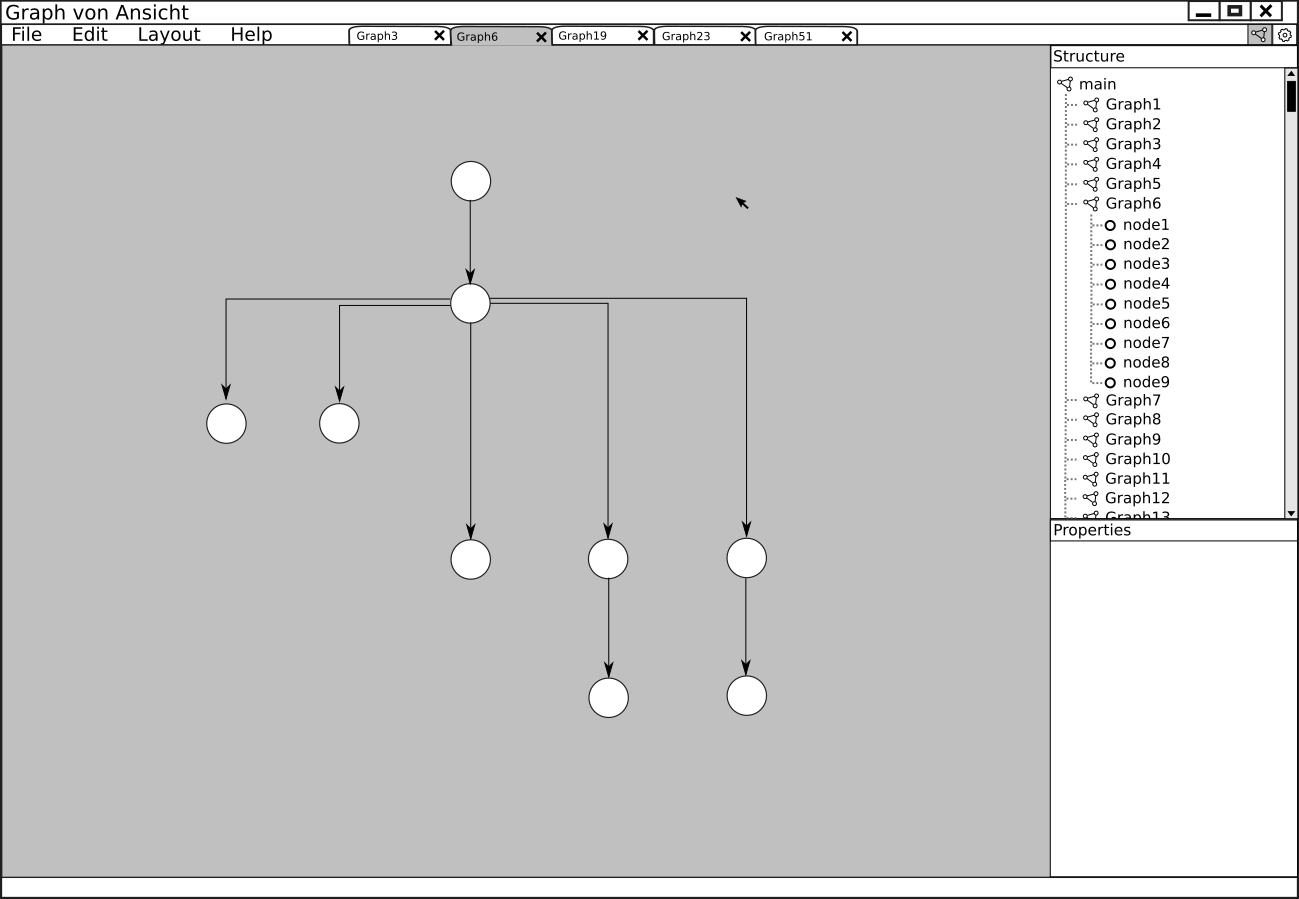
\includegraphics[width=380pt]{resourcen/gui_view_treeview.png}
  \caption{Hauptansicht}
  \label{fig:gui_view_treeview}
\end{figure}

\FloatBarrier

\begin{figure}[ht]
  \centering
  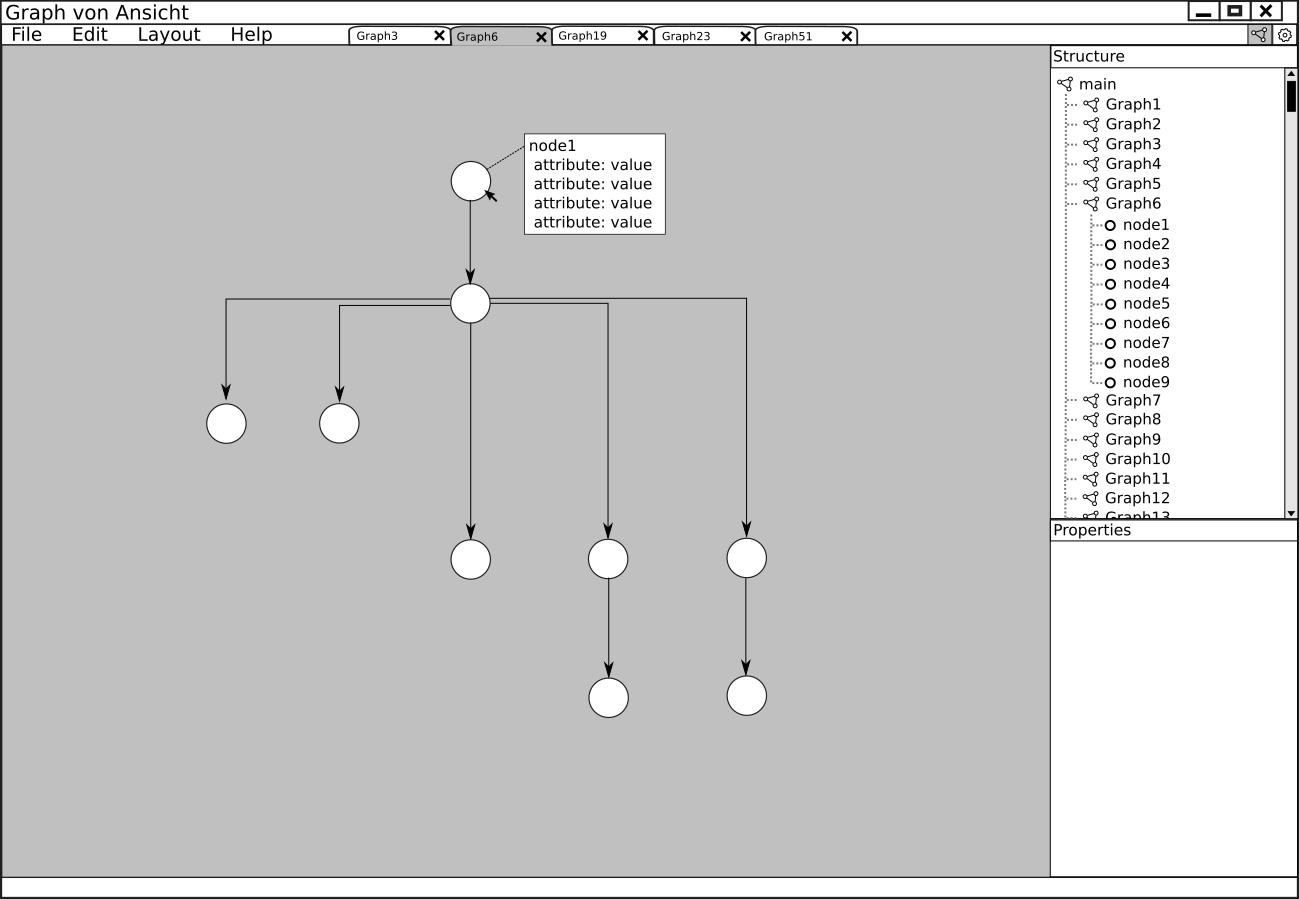
\includegraphics[width=380pt]{resourcen/gui_view_showInfoInView_node.png}
  \caption{Knoteninformation anzeigen}
  \label{fig:gui_view_showInfoInView_node}
\end{figure}

\begin{figure}[hb]
  \centering
  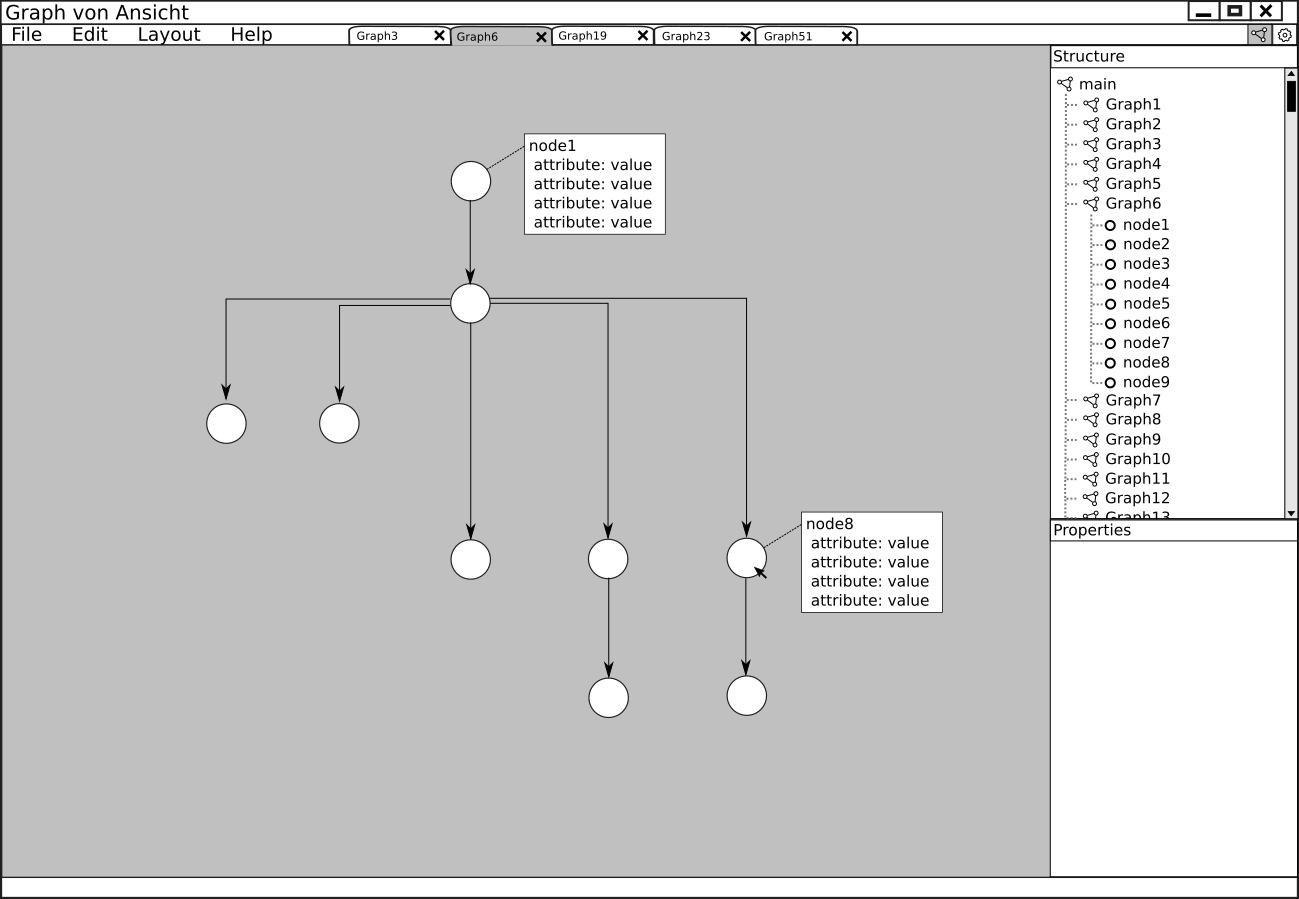
\includegraphics[width=380pt]{resourcen/gui_view_showInfoInView_node_multi.png}
  \caption{Mehrere Knoteninformationen anzeigen}
  \label{fig:gui_view_showInfoInView_node_multi}
\end{figure}

\begin{figure}[ht]
  \centering
  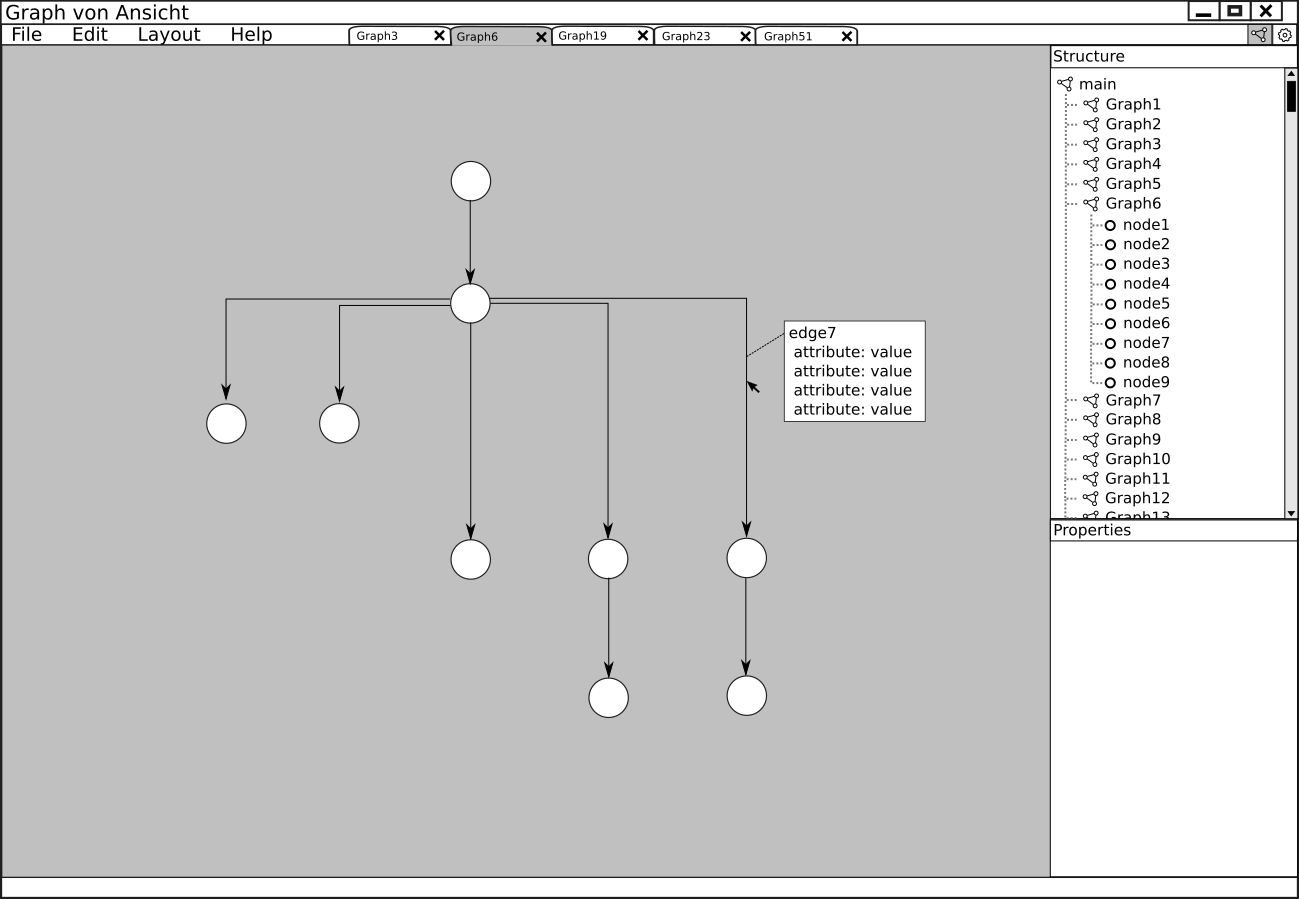
\includegraphics[width=380pt]{resourcen/gui_view_showInfoInView_edge.png}
  \caption{Kanteninformation Anzeigen}
  \label{fig:gui_view_showInfoInView_edge}
\end{figure}

\begin{figure}[hb]
  \centering
  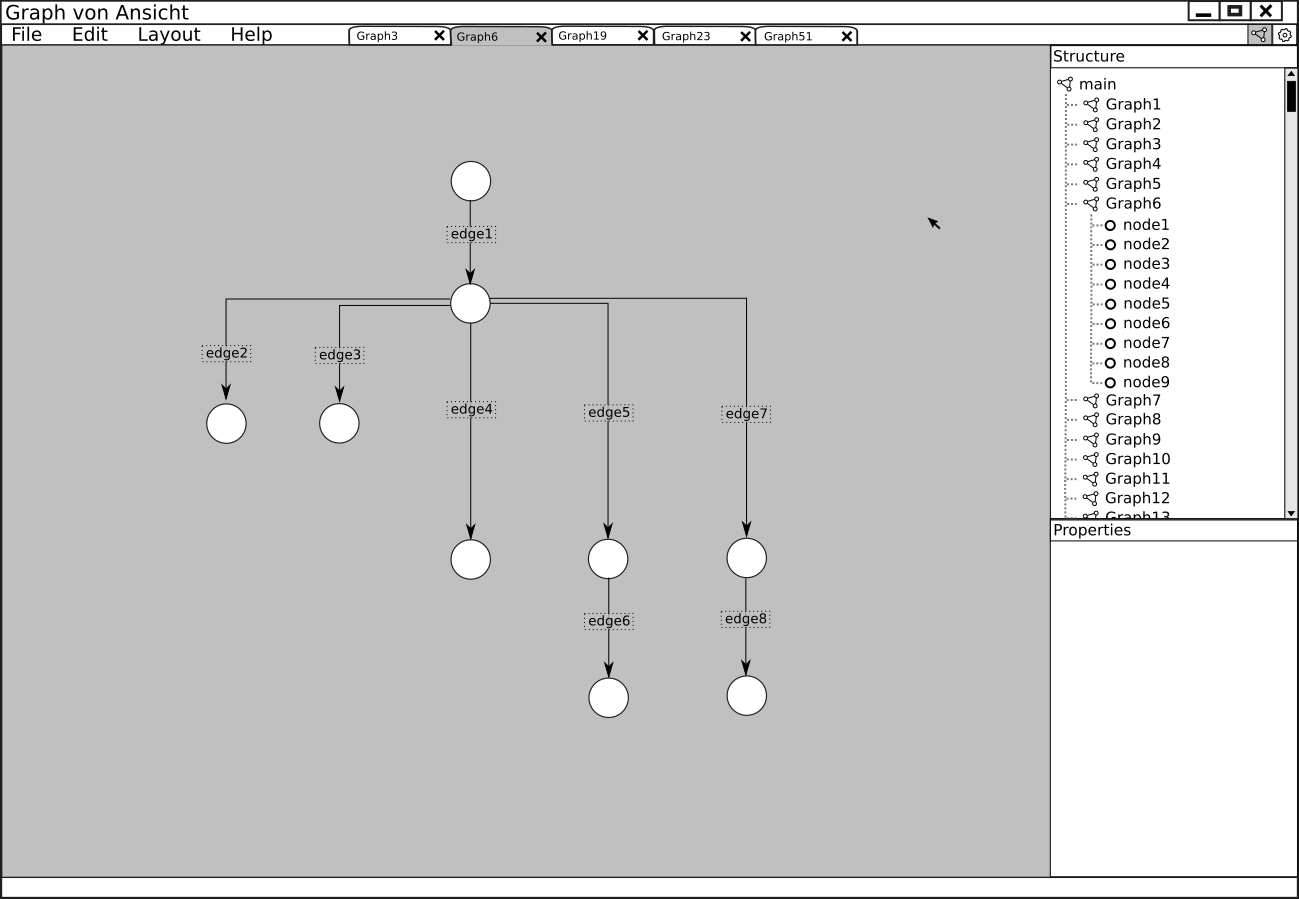
\includegraphics[width=380pt]{resourcen/gui_view_showInfoInView_edge_all.png}
  \caption{Anzeige aller Kantennamen}
  \label{fig:gui_view_showInfoInView_edge_all}
\end{figure}

\begin{figure}[ht]
  \centering
  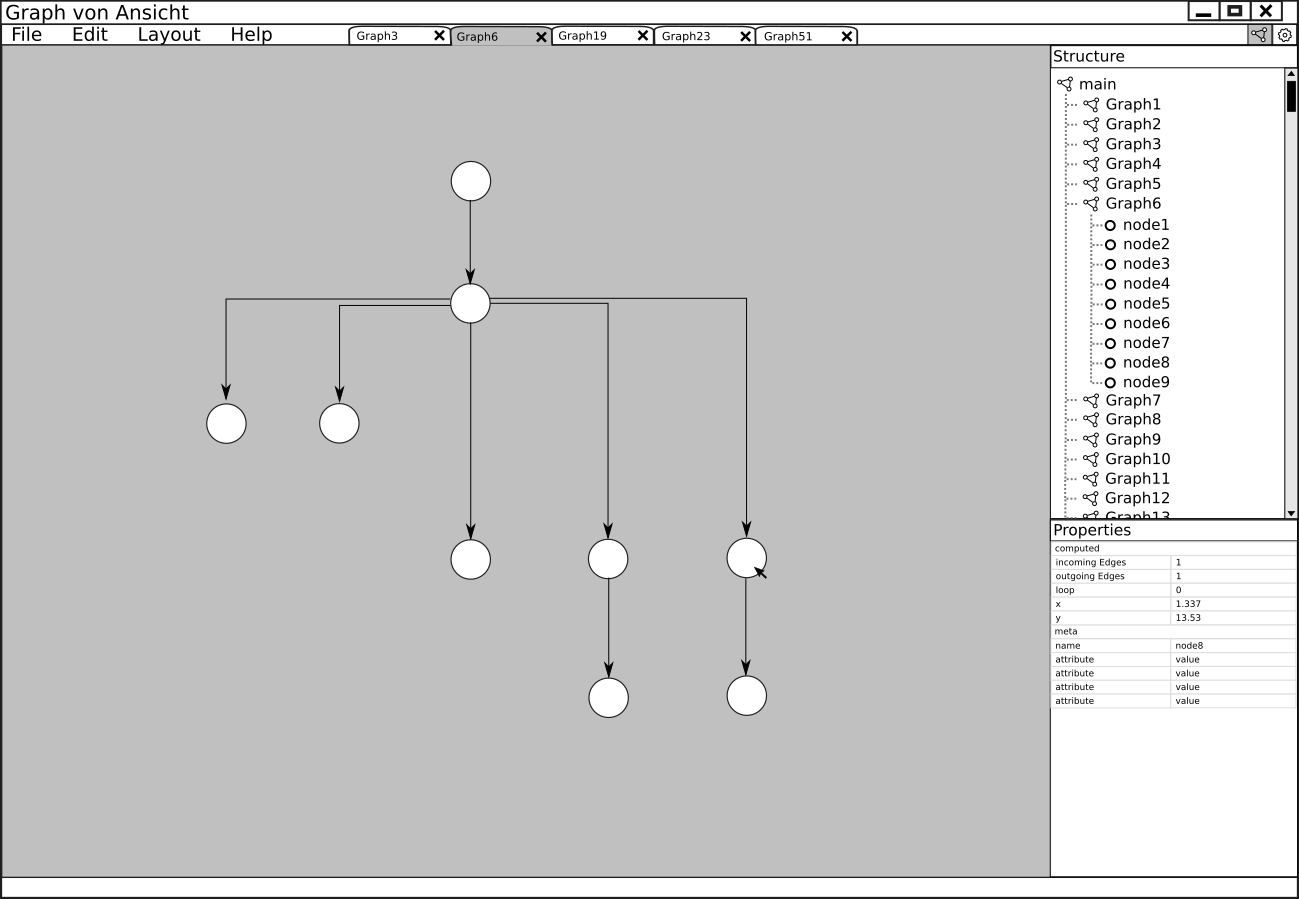
\includegraphics[width=380pt]{resourcen/gui_view_showInfoInProperties_node.png}
  \caption{Eigenschaftenansicht von Knoten}
  \label{fig:gui_view_showInfoInProperties_node}
\end{figure}

\begin{figure}[hb]
  \centering
  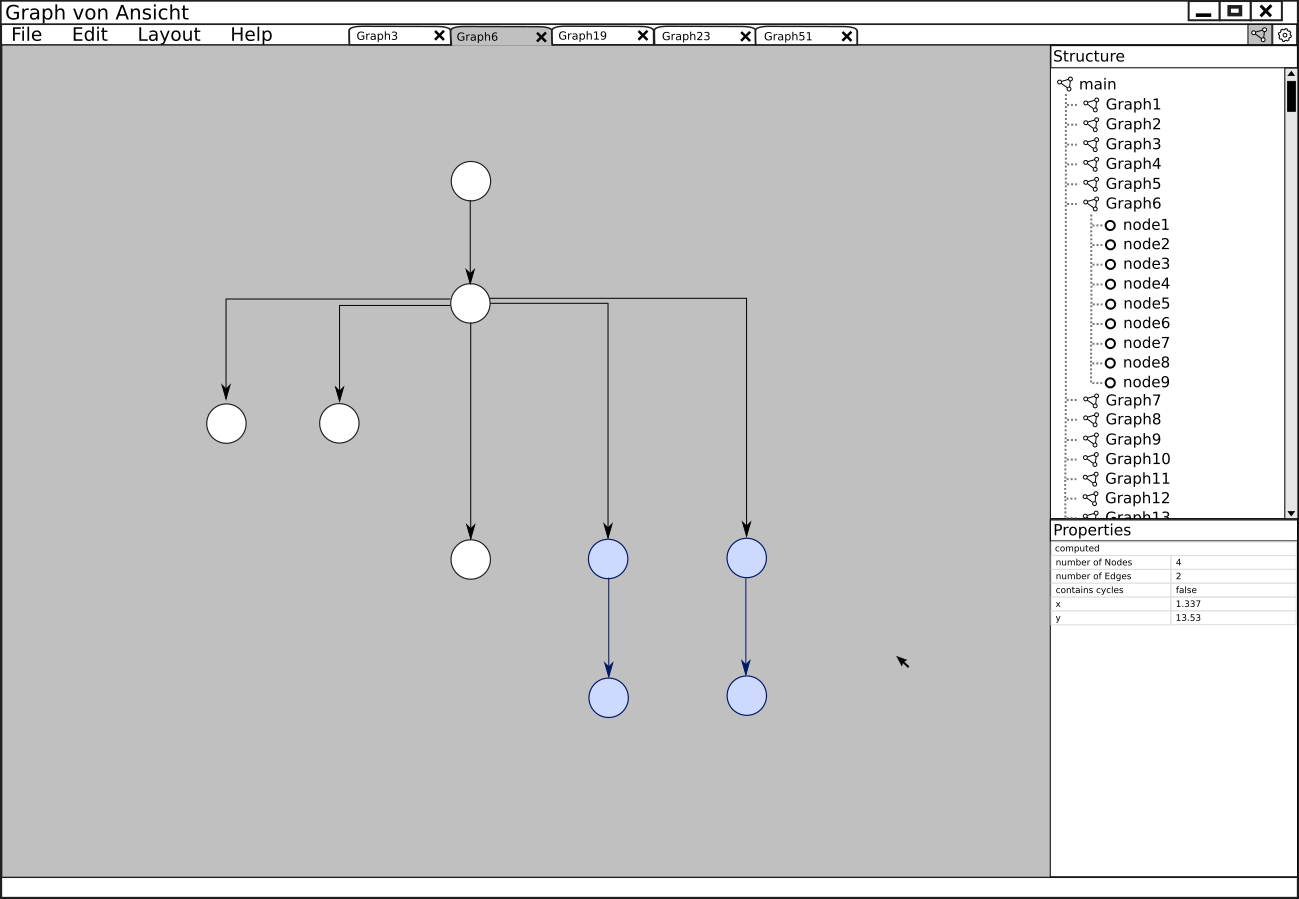
\includegraphics[width=380pt]{resourcen/gui_view_showInfoInProperties_multi.png}
  \caption{Eigenschaftenansicht von mehreren Knoten}
  \label{fig:gui_view_showInfoInProperties_multi}
\end{figure}

\begin{figure}[ht]
  \centering
  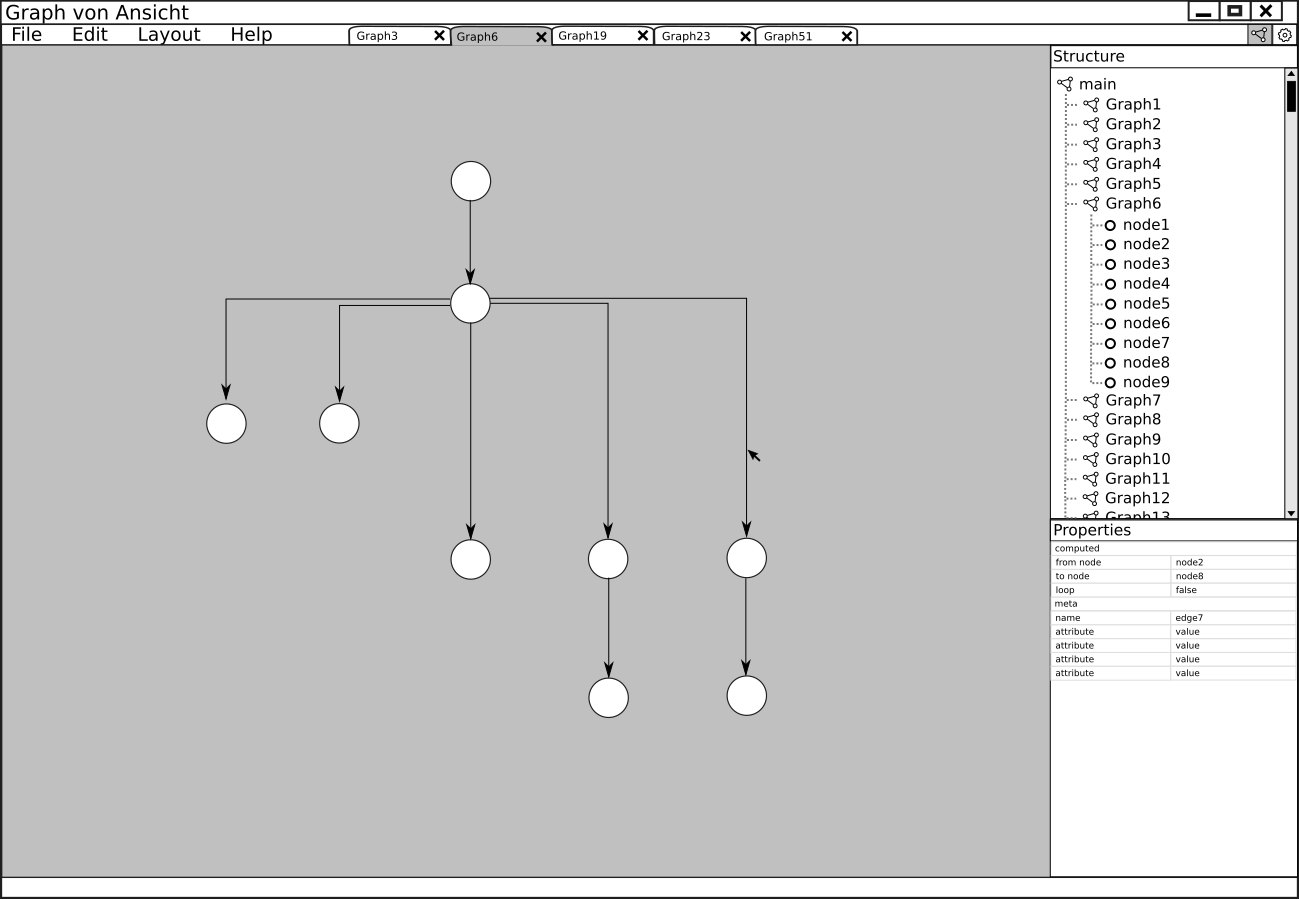
\includegraphics[width=380pt]{resourcen/gui_view_showInfoInProperties_edge.png}
  \caption{Eigenschaftenansicht von Ecken}
  \label{fig:gui_view_showInfoInProperties_edge}
\end{figure}

\begin{figure}[!ht]
  \centering
  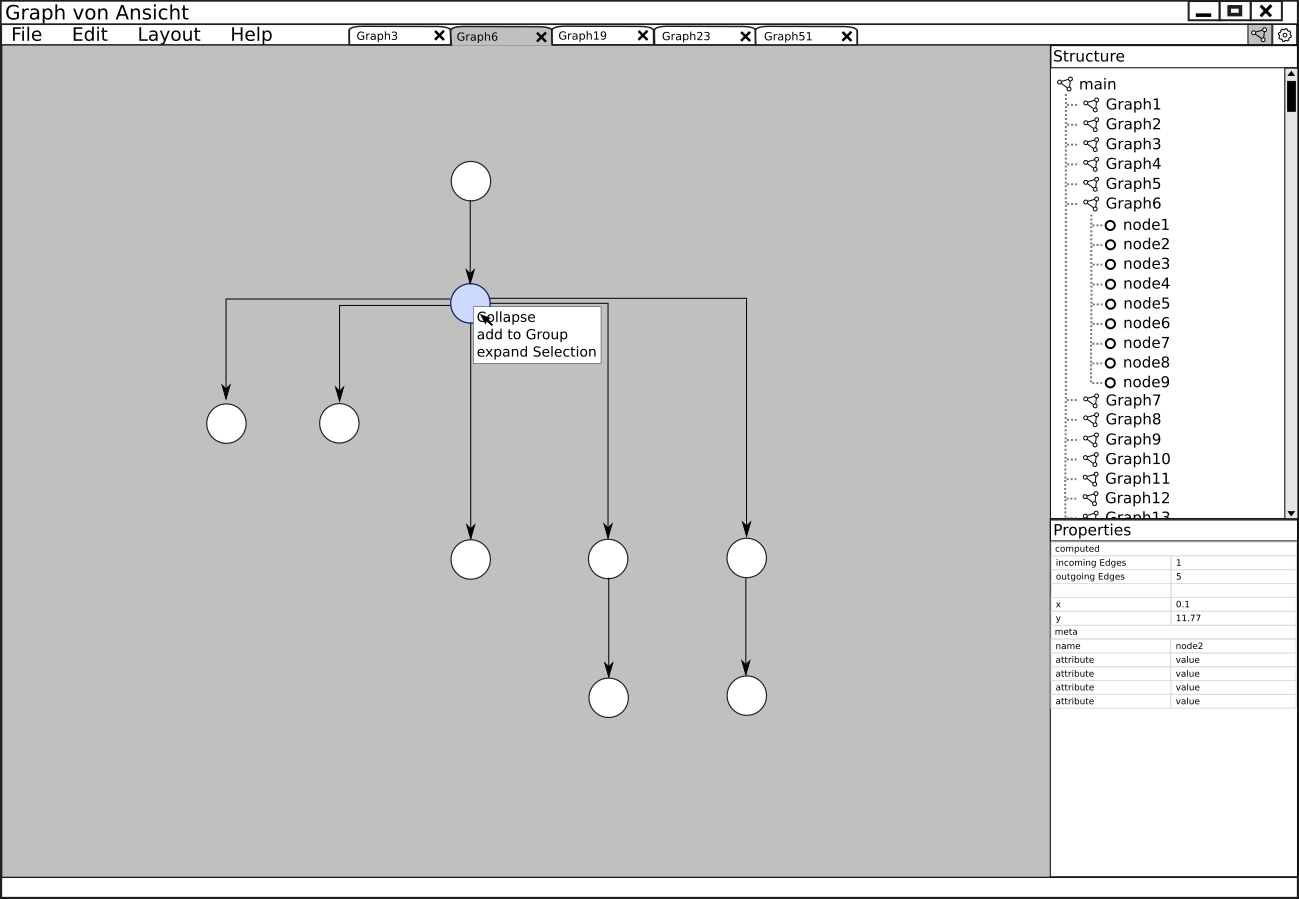
\includegraphics[width=380pt]{resourcen/gui_view_nodeMenu.png}
  \caption{Kontextmenü Knoten}
  \label{fig:gui_view_nodeMenu}
\end{figure}

\begin{figure}[!hb]
  \centering
  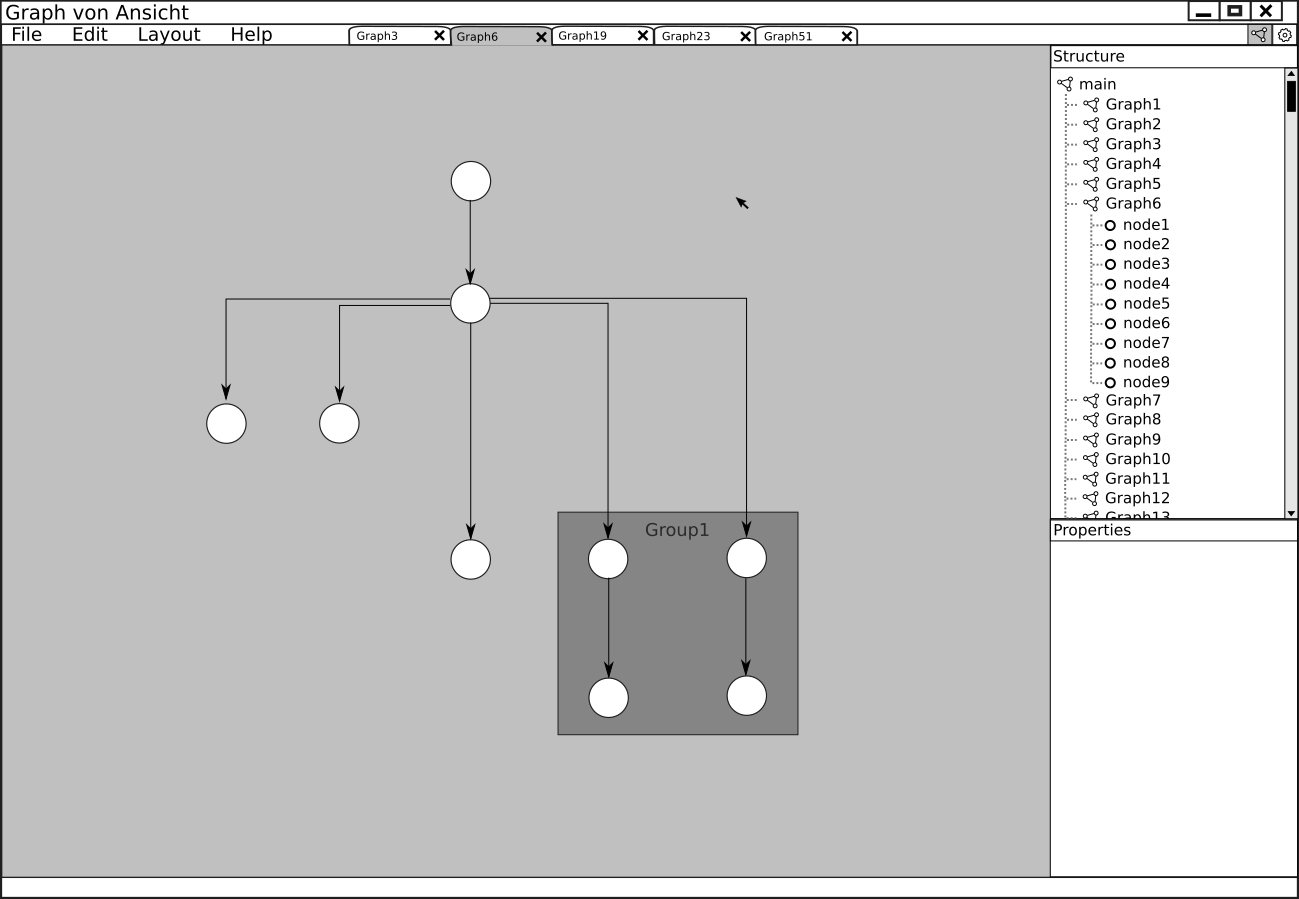
\includegraphics[width=380pt]{resourcen/gui_view_group.png}
  \caption{Gruppe von Knoten}
  \label{fig:gui_view_group}
\end{figure}

\FloatBarrier

\begin{figure}[hb]
  \centering
  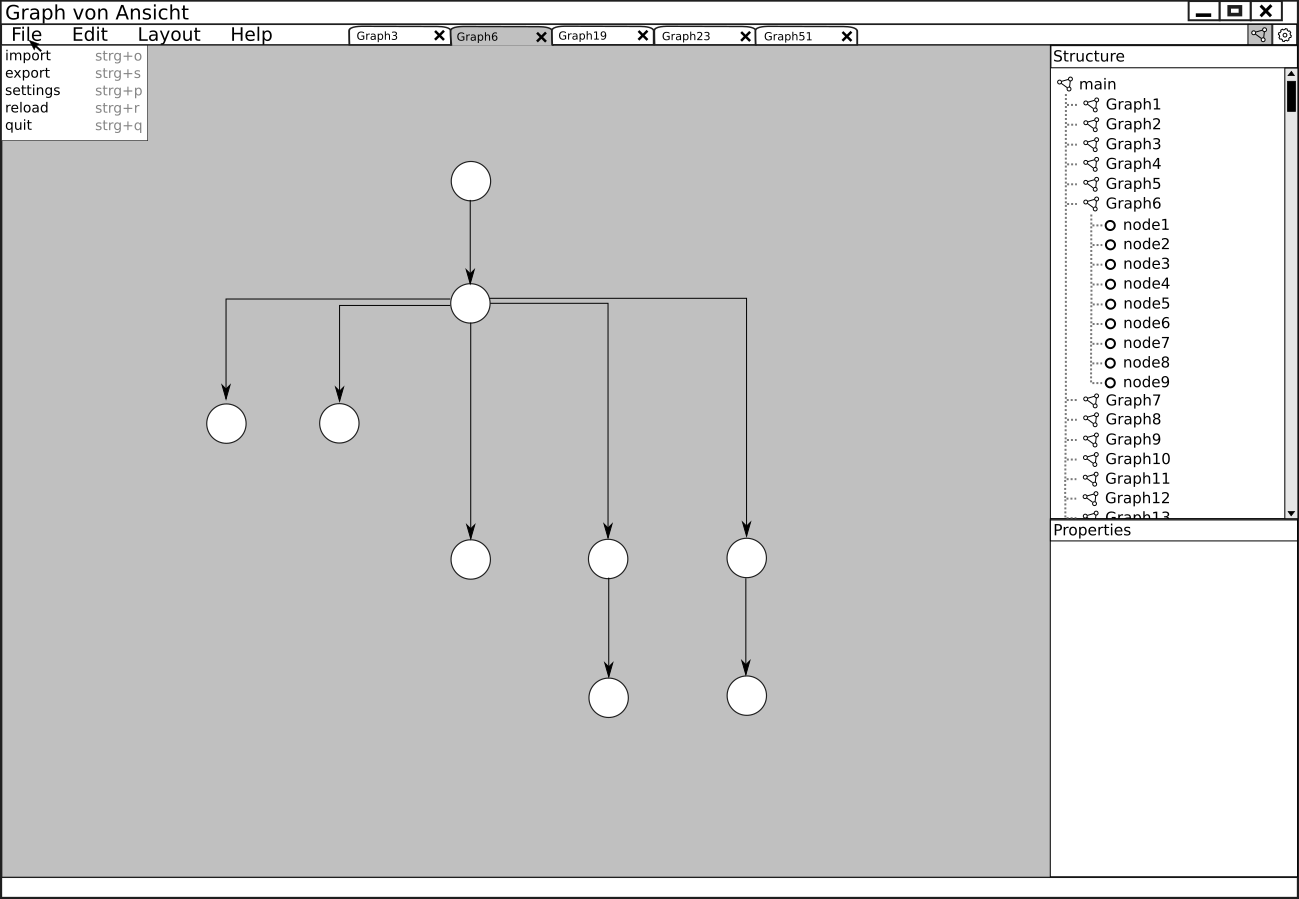
\includegraphics[width=380pt]{resourcen/gui_view_filemenu.png}
  \caption{Dateimenü}
  \label{fig:gui_view_filemenu}
\end{figure}

\begin{figure}[ht]
  \centering
  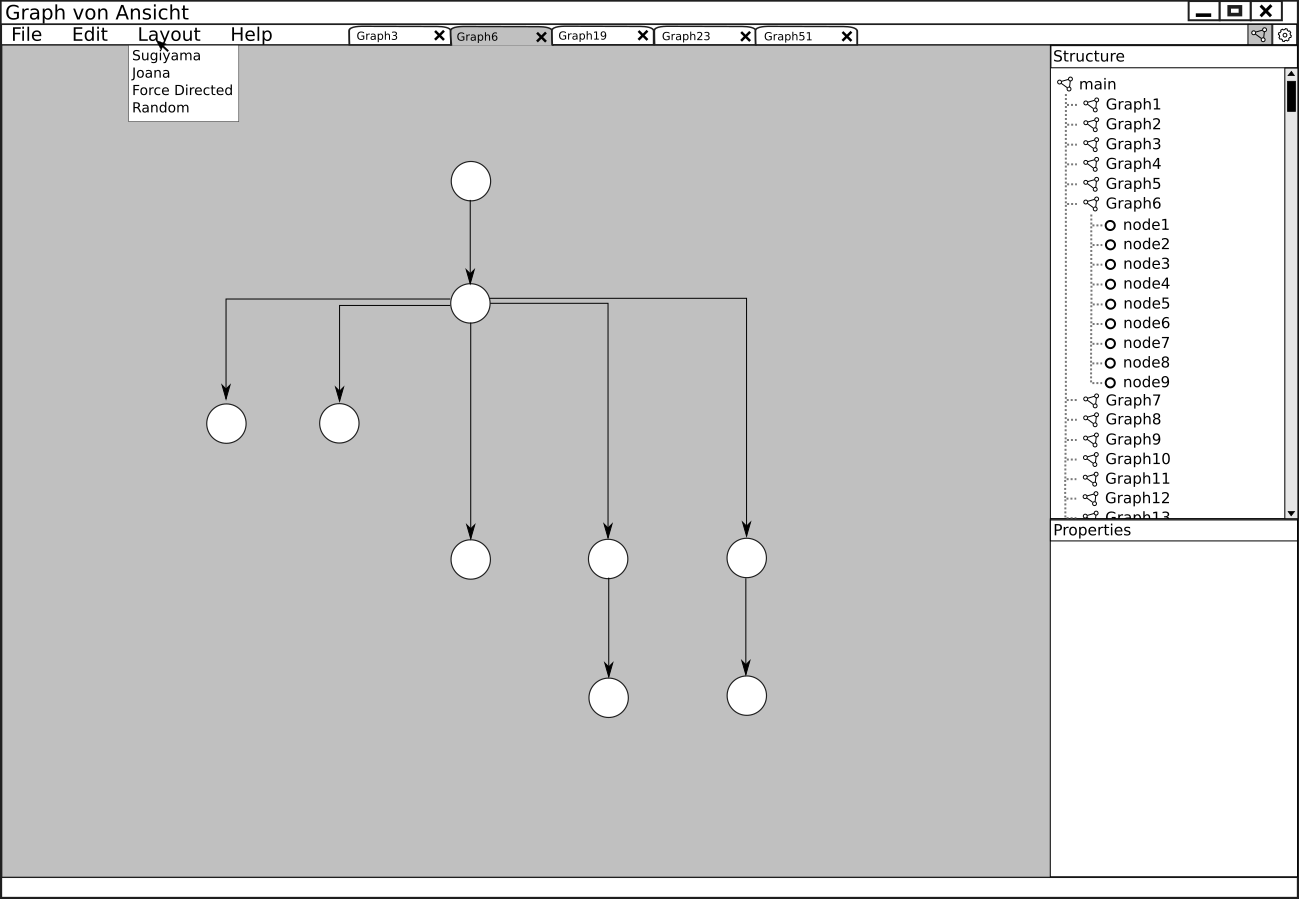
\includegraphics[width=380pt]{resourcen/gui_view_layoutmenu.png}
  \caption{Layoutmenü}
  \label{fig:gui_view_layoutmenu}
\end{figure}

\begin{figure}[hb]
  \centering
  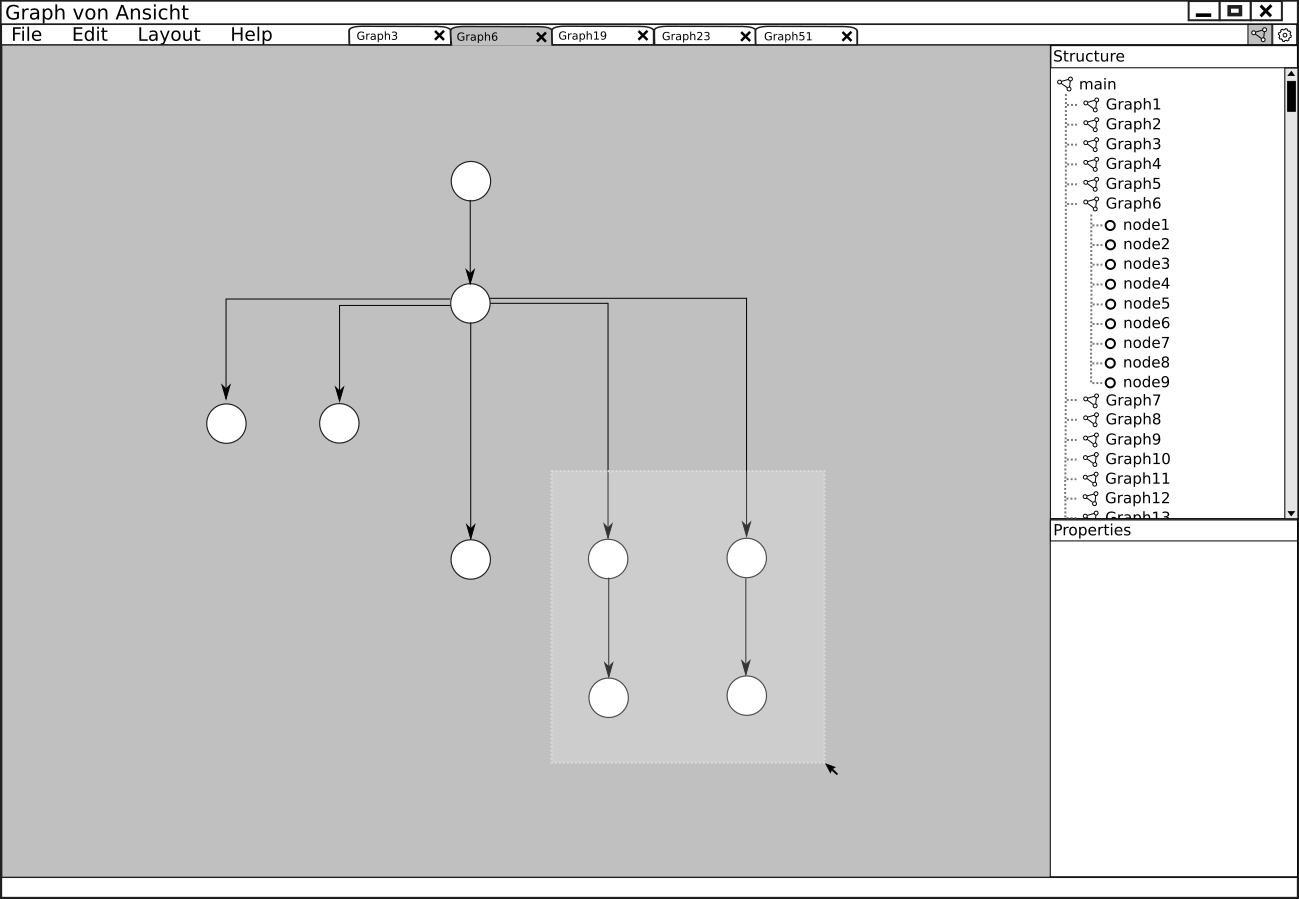
\includegraphics[width=380pt]{resourcen/gui_view_drawSelection.png}
  \caption{Auswahl mehrer Knoten und Kanten}
  \label{fig:gui_view_drawSelection}
\end{figure}

\begin{figure}[ht]
  \centering
  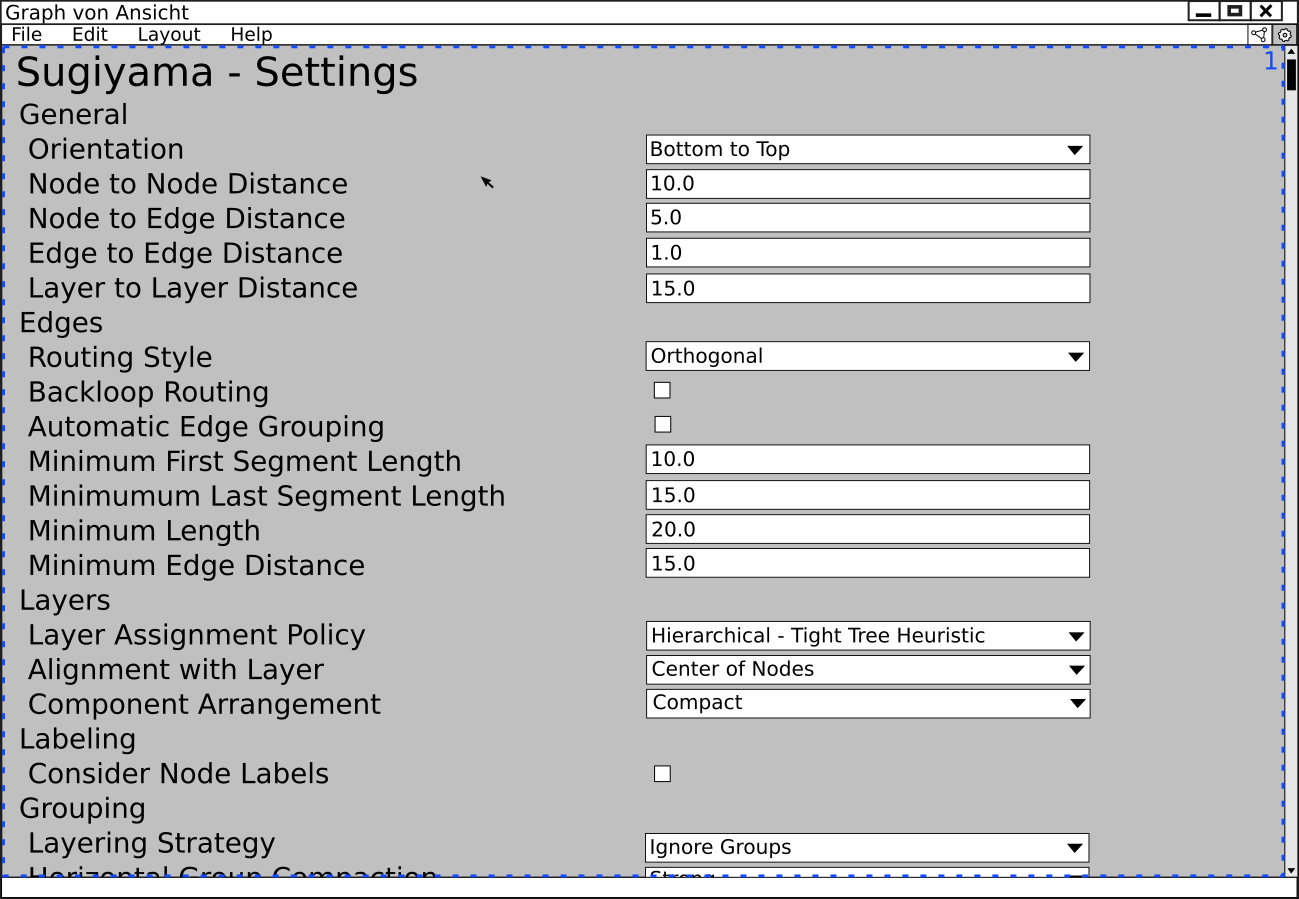
\includegraphics[width=380pt]{resourcen/gui_layoutsettings_settings.png}
  \caption{Einstellungen des Layoutalgorithmus}
  \label{fig:gui_layoutsettings_settings}
\end{figure}

\begin{figure}[hb]
  \centering
  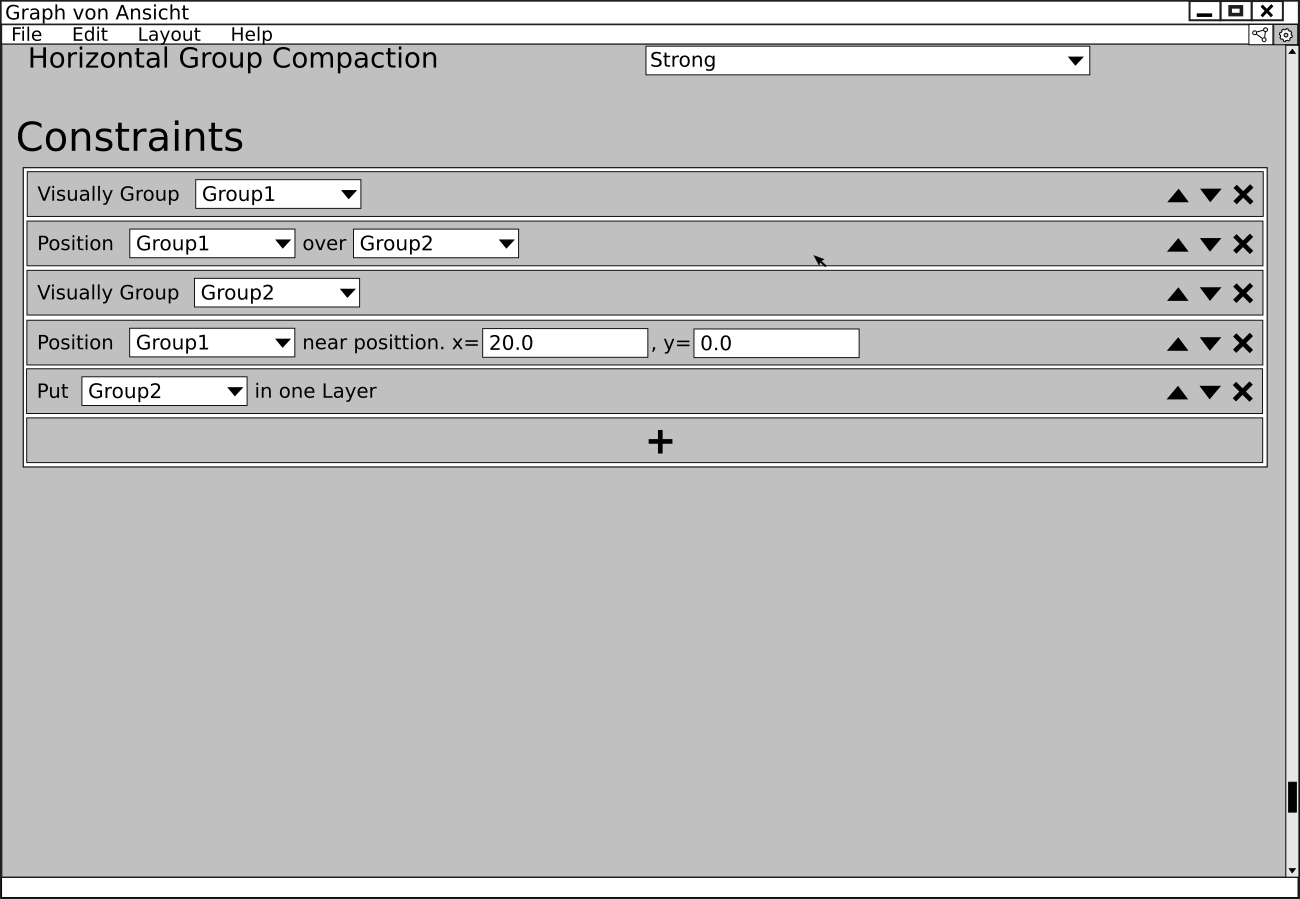
\includegraphics[width=380pt]{resourcen/gui_layoutsettings_constraints.png}
  \caption{Einstellungen der Layout Constraints}
  \label{fig:gui_layoutsettings_constraints}
\end{figure}

\begin{figure}[ht]
  \centering
  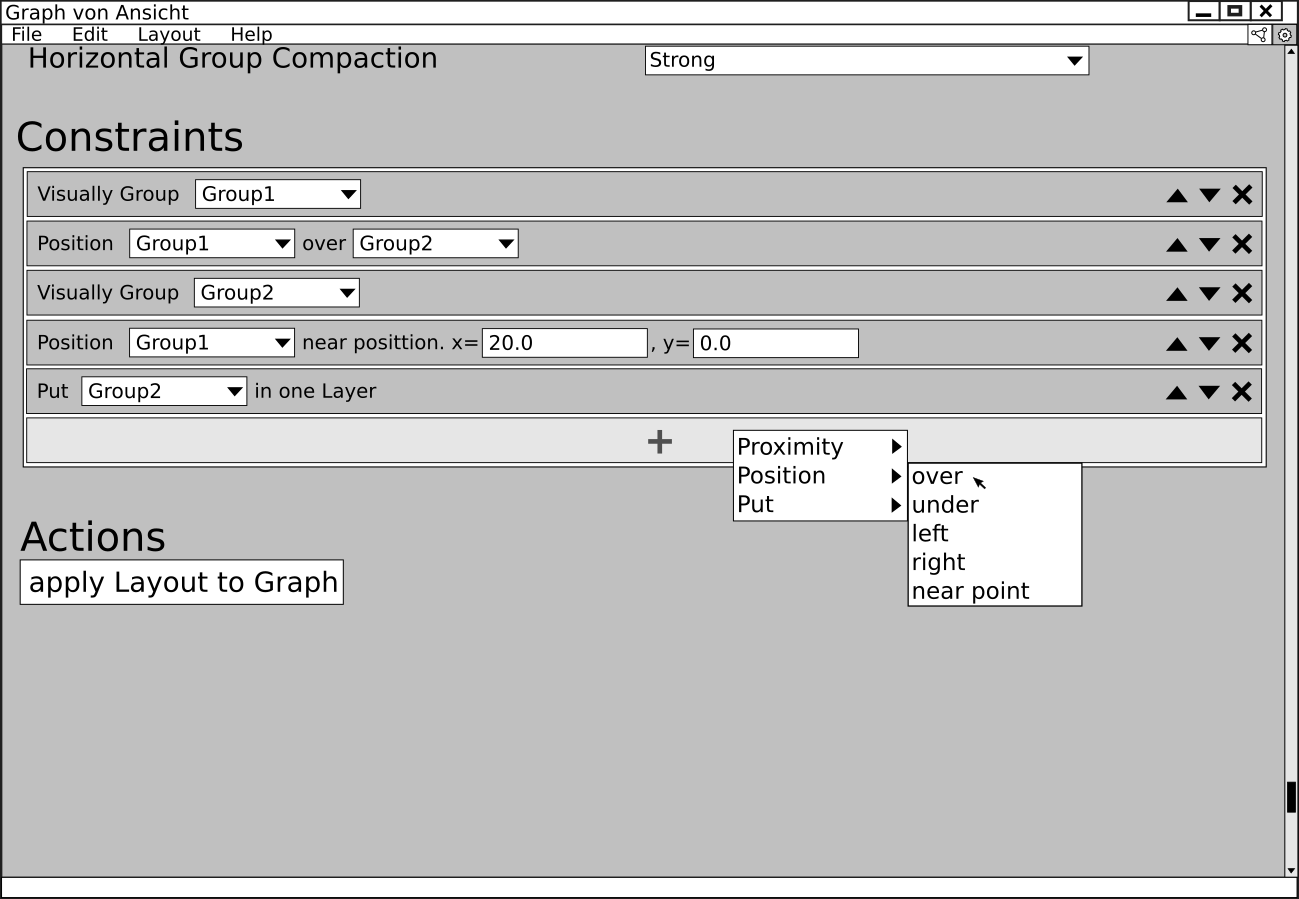
\includegraphics[width=380pt]{resourcen/gui_layoutsettings_constraints_new.png}
  \caption{neues Constraint hinzufügen}
  \label{fig:gui_layoutsettings_constraints_new}
\end{figure}

\begin{figure}[hb]
  \centering
  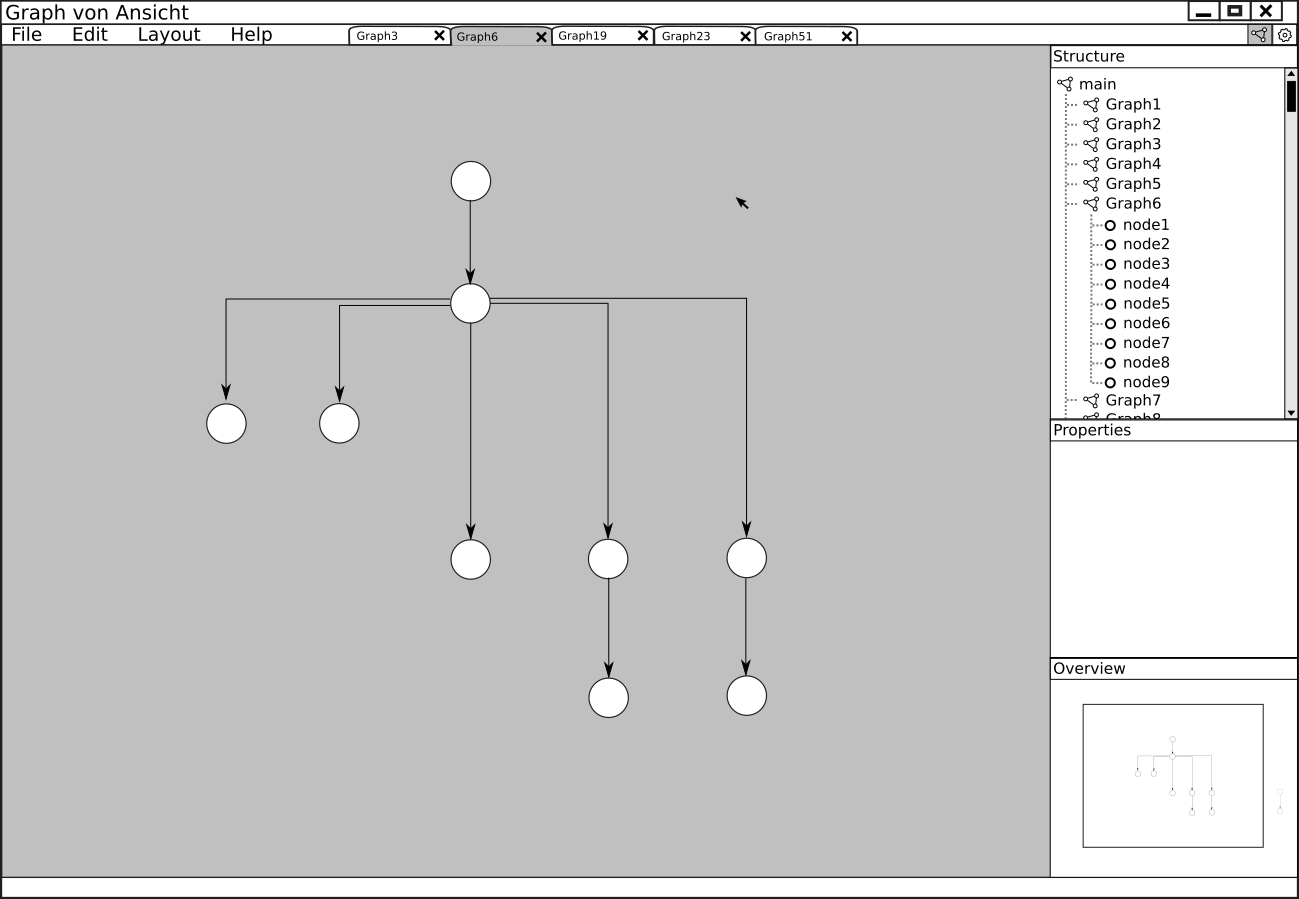
\includegraphics[width=380pt]{resourcen/gui_view_minimap.png}
  \caption{Übersichtsanzeige des aktuellen Graphen}
  \label{fig:gui_view_minimap}
\end{figure}

\begin{figure}[ht]
  \centering
  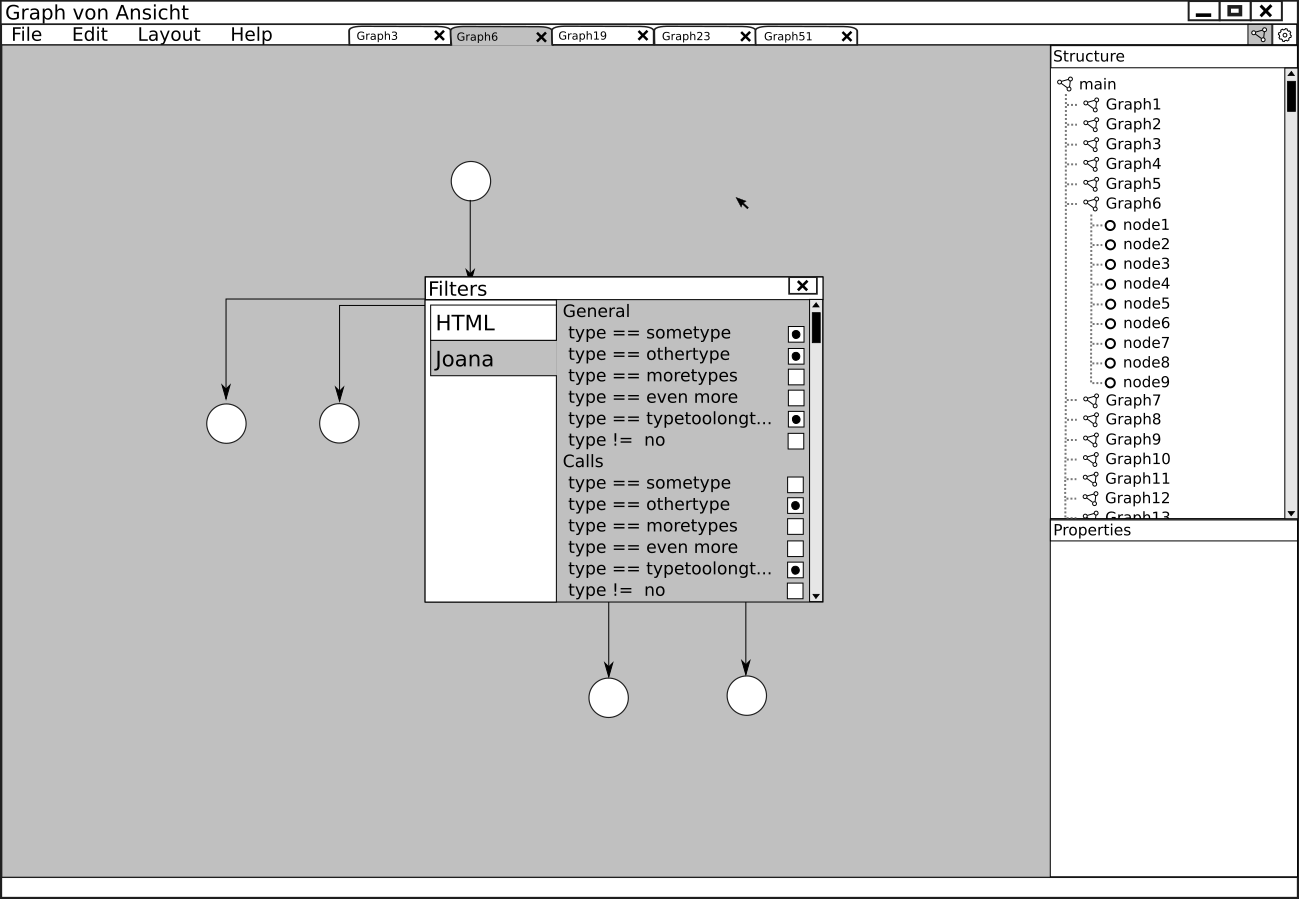
\includegraphics[width=380pt]{resourcen/gui_window_filters.png}
  \caption{Filtereinstellungen}
  \label{fig:gui_window_filters}
\end{figure}

\begin{figure}[hb]
  \centering
  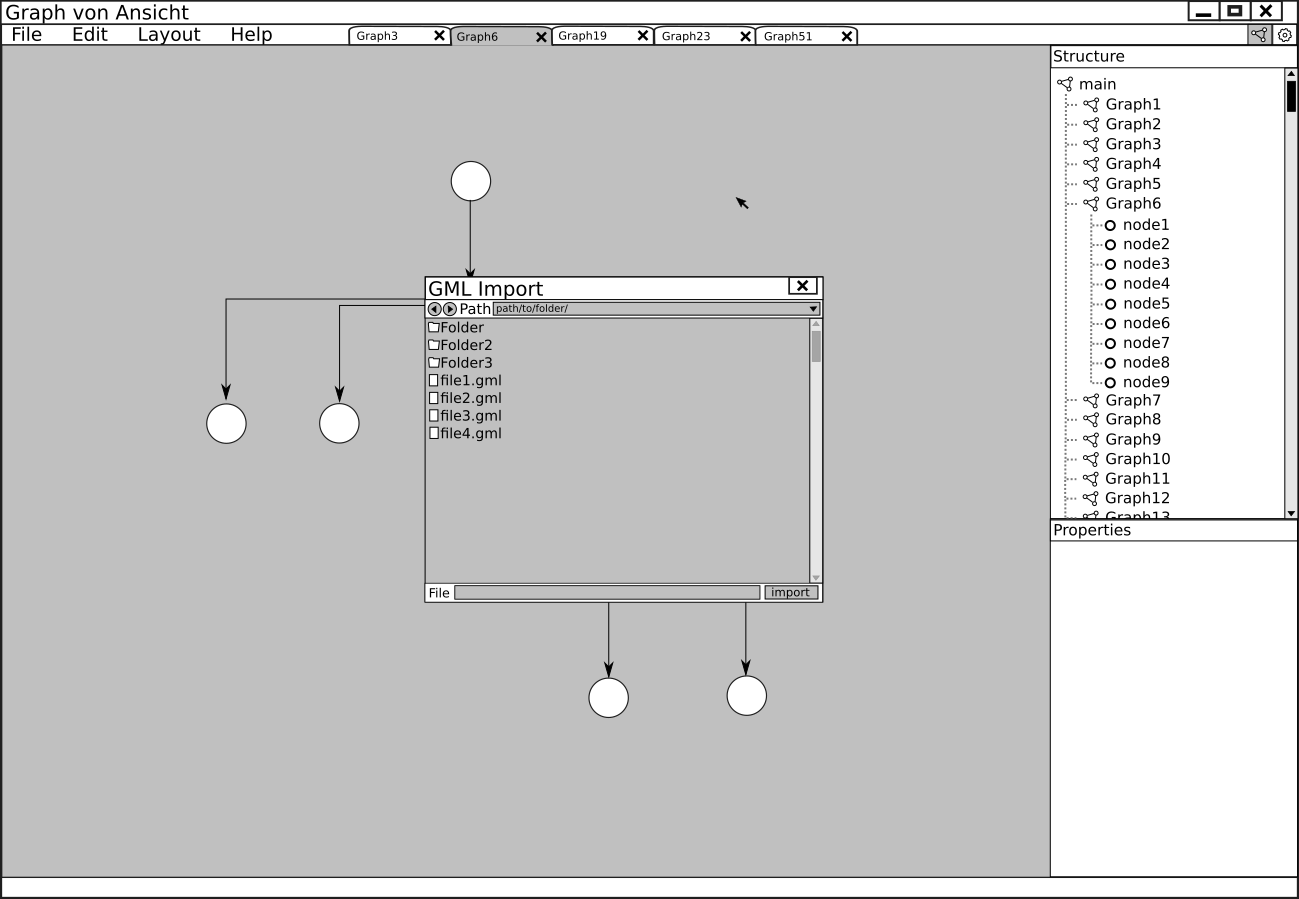
\includegraphics[width=380pt]{resourcen/gui_window_import.png}
  \caption{Importieren einer Datei}
  \label{fig:gui_window_import}
\end{figure}

\begin{figure}[ht]
  \centering
  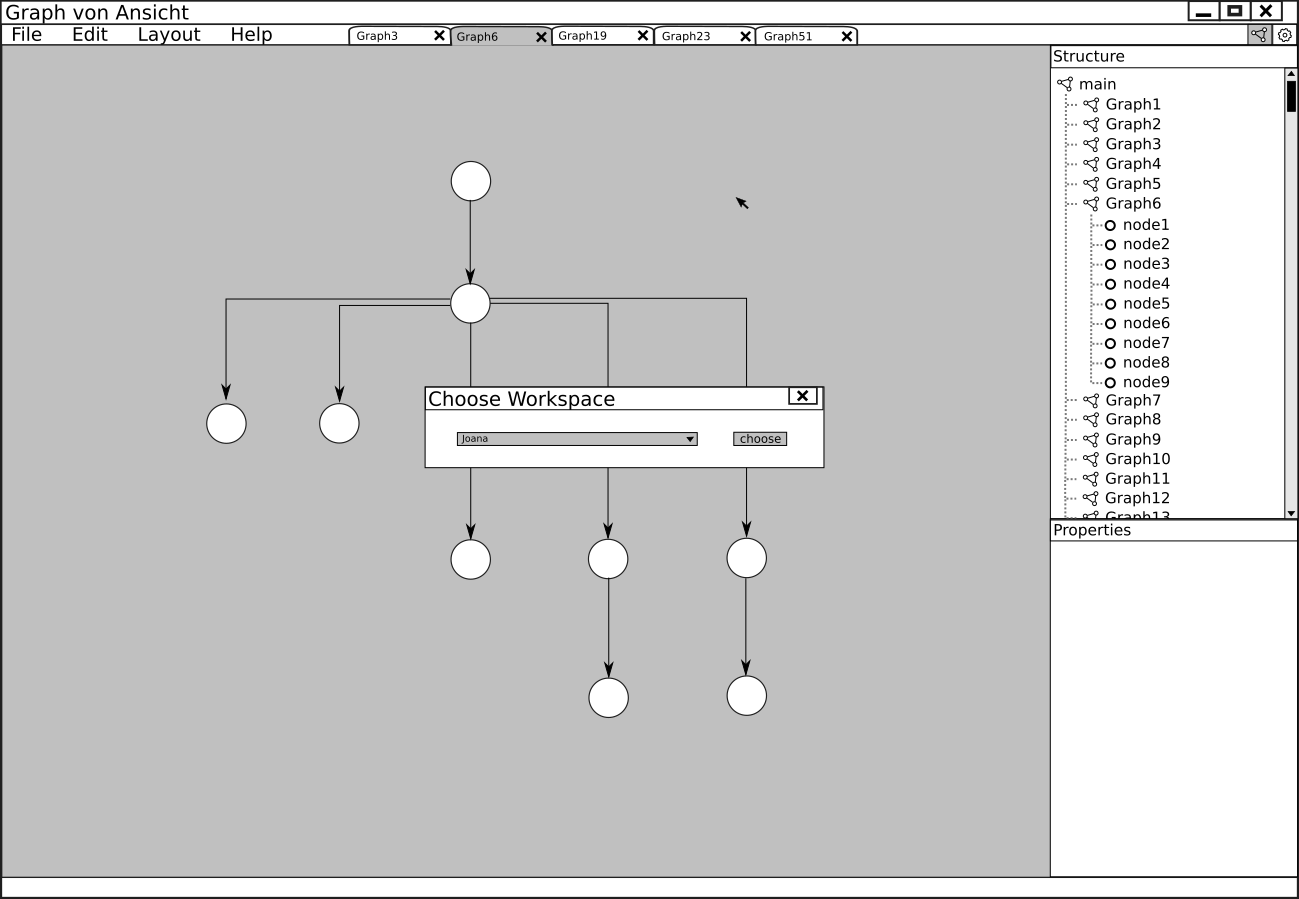
\includegraphics[width=380pt]{resourcen/gui_window_chooseWorkspace.png}
  \caption{Arbeitsbereich auswählen}
  \label{fig:gui_window_chooseWorkspace}
\end{figure}



\chapter{Globale Testfälle}

\setcounter{tnr}{10}
\newcommand{\testno}{\ifnum\value{tnr}<10 00\else\ifnum\value{tnr}<100 0\fi\fi\arabic{tnr}\addtocounter{tnr}{10}}
\newcommand\test[2]{\namedlabel{test:#1}{\textbf{/T\testno/}}: & #2 \\ [1ex] }
\newcommand\etest[3]{\namedlabel{test:#1}{\textbf{/T\testno/}}: & #2 \\ & Erweiterung: #3 \\ [1ex] }

%TODO: Siehe im Tips Dokument für Beispiel für richtige Testfälle. Die Wichtigsten Funkt. anforderungen testen.
\begin{tabular}{lp{0.9\linewidth}}
  \test{start}{Das Programm wird vom Tester gestartet.
    Es wird überprüft, ob sich die GUI öffnet und, wie in \ref{ch:gui} beschrieben, dargestellt wird.}
  \etest{startcmd}{Das Programm wird vom Tester über die Kommandozeile geöffnet.
    Die Graphdatei wird als Argument mitübergeben.
    Wie in \ref{test:start} wird die korrekte Darstellung der GUI überprüft.
    Zusätzlich wird getestet, ob der(die) Graph(en) aus der Graphdatei korrekt geladen werden. \ref{fa:import}}
    {Alle möglichen validen Kombinationen von zusätzlichen Argumenten, beschrieben in \ref{sec:uicmd}, werden ausprobiert.
    Außerdem werden auch invalide Argumente übergeben und überprüft \ref{nfa:gracefulexit} eingehalten wird.}
  \test{import}{Der Tester wählt über die Menüleiste eine Import-Möglichkeit aus.
    Es wird überprüft ob, die GUI die Anfrage, wie in \ref{fa:import} beschrieben,
    behandelt und, ob die Graphen in der Graphdatei in der Graph-Übersicht gelistet werden.}
  \test{export}{Ein Graph ist in der Graphansicht geladen.
    Der Tester wählt über die Menüleiste eine Export-Möglichkeit.
    Es wird überprüft, ob die GUI die Anfrage, wie in \ref{fa:export_img} beschrieben,
    behandelt und ob die exportierte Bilddatei mit der in der Graphansicht dargestellten Visualisierung des Graphen übereinstimmt.}
  \test{layouten}{Der Tester wählt über die Menüleiste eine Layout-Möglichkeit aus.
    Es wird überprüft, ob das Layout auf den Graphen umgesetzt wird \ref{fa:layout}
    und die Zeitbedingungen \ref{nfa:berechzeit} eingehalten werden.
    Für den Fall, dass JOANA-Layout ausgewählt wurde,
    werden zusätzlich alle Nichtfunktionalen Anforderungen für das \nameref{sec:nfajoana} überprüft.}
  \test{navigation}{Der Tester führt alle in \ref{fa:zoom} \ref{fa:verschieben} beschriebene Navigationsaktionen aus
    und überprüft, ob das Produkt sich wie in den Anforderungen beschrieben verhält.}
  \test{filter}{Ein Graph ist in der Graphansicht geladen.
    Der Tester wählt eine Filter-Funktion aus der Menüleiste aus.
    Es wird überprüft, ob genau die Knoten ausgeblendet bzw. wieder eingeblendet werden, welche das Filterkriterium erfüllen.}
\end{tabular}


\chapter{Systemmodelle}
\label{ch:sysmodel}

\section{Allgemeine Modelle}
\begin{figure}[ht]
	\centering
	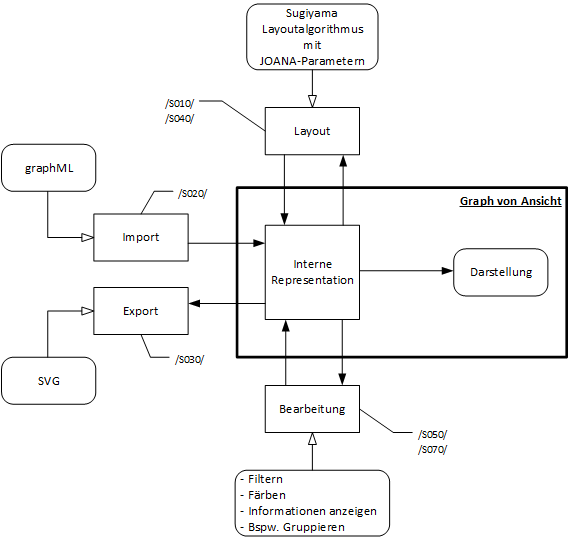
\includegraphics[width=360pt]{resourcen/plugin.png}
	\caption{Programmaufbau und Datenfluss}
	\label{fig:aufbaudatenfluss}
\end{figure}
\newpage
\section{Anwendungsfälle}
\begin{figure}[ht]
	\centering
	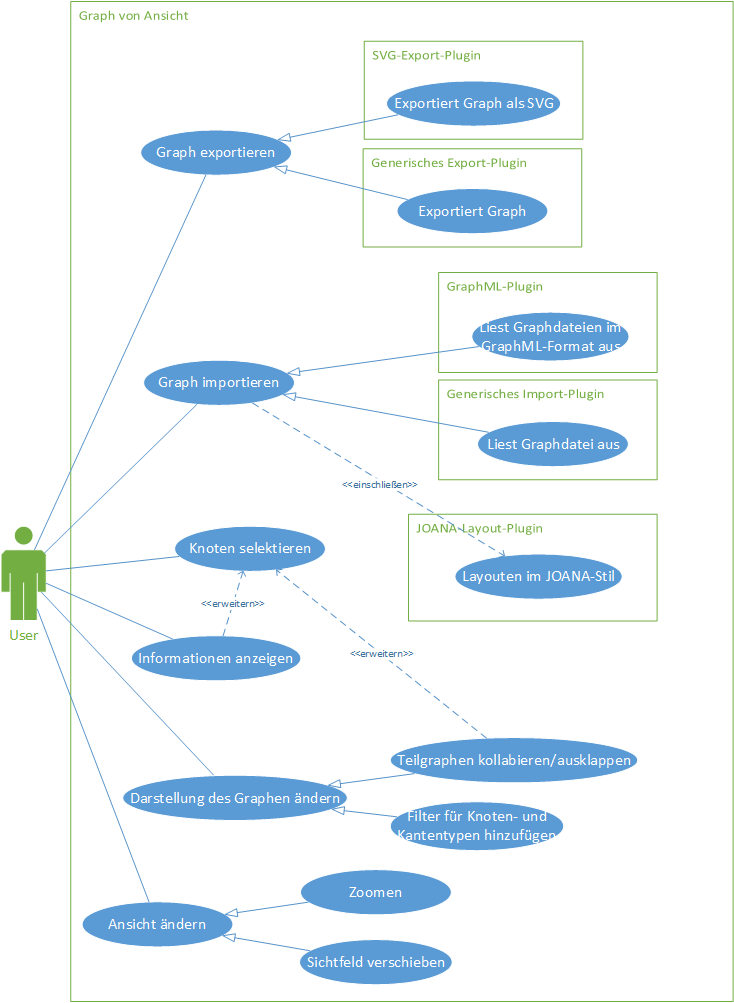
\includegraphics[width=310pt]{resourcen/usecase.png}
	\caption{Anwendungsfalldiagramm}
	\label{fig:usecase}
\end{figure}

\clearpage
\printglossary[type=\acronymtype]
\printglossary[title=Glossar,toctitle=Glossar]

\listoffigures

\end{document}
